% cd /disks/PROJECT/Mickael/COMMUNICATION/CST2015/;
% pdflatex THESE_CST2015.tex; bibtex THESE_CST2015; pdflatex THESE_CST2015.tex; pdflatex THESE_CST2015.tex;
% evince THESE_CST2015.pdf &

\documentclass[11pt, a4paper]{article}
\documentclass[11pt, a4paper]{article}
\pdfpageattr{/Group << /S /Transparency /I true /CS /DeviceRGB>>}

\usepackage[T1]{fontenc}
\usepackage[utf8]{inputenc}
\usepackage{graphicx}
\usepackage[usenames, dvipsnames, svgnames, x11names, hyperref, RGB]{xcolor}
\usepackage{tabularx}
\usepackage{multirow}
\usepackage{pifont}
\usepackage{multicol}
\usepackage{setspace}
\renewcommand{\baselinestretch}{1.5}
\usepackage{helvet}
\renewcommand{\familydefault}{\sfdefault}

\usepackage{longtable}
\usepackage[format=plain, font=normalsize, labelfont=bf, hang]{caption}
\usepackage[hmargin=2.5cm, vmargin=2.5cm]{geometry}
\usepackage{amsmath}
\usepackage{indentfirst} % add indent in first paragraph


\usepackage{fancyhdr}
\pagestyle{fancy}
\fancyhead[L]{\slshape \rightmark}
% \fancyhead[R]{\slshape \leftmark}
% \fancyhead[L]{\today}

\usepackage{helvet}
\renewcommand{\familydefault}{\sfdefault}

\definecolor{dodgerblue}{RGB}{30,144,255}
\definecolor{springgreen3}{RGB}{0,139,69}
% \definecolor{springgreen2}{RGB}{0,205,102}
\definecolor{firebrick2}{RGB}{238,44,44}
\definecolor{maroon2}{RGB}{238,48,167}
\definecolor{goldenrod2}{RGB}{238,180,34}
\definecolor{deepskyblue}{RGB}{0,191,255}

\usepackage{textcomp}
\usepackage{listings}
\usepackage{courier}
\lstset{ %
    backgroundcolor=\color{dodgerblue!2.5!white},       % choose the background color; you must add \usepackage{color} or \usepackage{xcolor}
    basicstyle={\tiny\ttfamily\mdseries},               % the size of the fonts that are used for the code
    breakatwhitespace=true,                             % sets if automatic breaks should only happen at whitespace
    breaklines=true,                                    % sets automatic line breaking
    captionpos=t,                                       % sets the caption-position to bottom
    commentstyle=\color{springgreen3},                  % comment style
    deletekeywords={...},                               % if you want to delete keywords from the given language
    escapeinside={!*}{*!},                              % if you want to add LaTeX within your code
    extendedchars=true,                                 % lets you use non-ASCII characters; for 8-bits encodings only, does not work with UTF-8
    frame=single,                                       % adds a frame around the code
    keepspaces=true,                                    % keeps spaces in text, useful for keeping indentation of code (possibly needs columns=flexible)
    keywordstyle={\color{dodgerblue}\textbf},           % keyword style
    morekeywords={*,...},                               % if you want to add more keywords to the set
    numbers=none,                                       % where to put the line-numbers; possible values are (none, left, right)
    numbersep=10pt,                                     % how far the line-numbers are from the code
    numberstyle=\tiny\color{goldenrod2},                % the style that is used for the line-numbers
    rulecolor=\color{dodgerblue},                       % if not set, the frame-color may be changed on line-breaks within not-black text (e.g. comments (green here))
    showspaces=false,                                   % show spaces everywhere adding particular underscores; it overrides 'showstringspaces'
    showstringspaces=false,                             % underline spaces within strings only
    showtabs=false,                                     % show tabs within strings adding particular underscores
    stepnumber=1,                                       % the step between two line-numbers. If it's 1, each line will be numbered
    stringstyle=\color{maroon2},                        % string literal style
    tabsize=2,                                          % sets default tabsize to 2 spaces
    title=\lstname,                                     % show the filename of files included with \lstinputlisting; also try caption instead of title
    showlines=false,                                    % prints empty lines at the end of listings
    xleftmargin=9mm,                                    % The dimensions are used as extra margins on the left and right
    xrightmargin=9mm,
    upquote=true,
    lineskip=-0.05ex,                                   % Specifies additional space between lines in listings
    aboveskip=0ex,                                      % Define the space above and below displayed listings
    belowskip=0ex,                                      % Define the space above and below displayed listings
}
\lstdefinelanguage{JuliaConsole}{
    backgroundcolor=\color{gray!2.5!white},             % choose the background color; you must add \usepackage{color} or \usepackage{xcolor}
    rulecolor=\color{gray!50!white},                    % if not set, the frame-color may be changed on line-breaks within not-black text (e.g. comments (green here))
    alsoletter={>},
    literate=%
    *{\$}{{{\color{black}\bfseries \$}}}1
    {julia>}{{{\color{black}\bfseries julia>}}}6
}
\lstdefinelanguage{Julia}{
    keywordsprefix=\@,
    morekeywords={
        exit, whos, edit, load, is, isa, isequal, typeof, tuple, ntuple, uid, hash, finalizer, convert, promote,
        subtype, typemin, typemax, realmin, realmax, sizeof, eps, promote_type, method_exists, applicable,
        invoke, dlopen, dlsym, system, error, throw, assert, new, Inf, Nan, pi, im, begin, while, for, in, return,
        break, continue, macro, quote, let, if, elseif, else, try, catch, end, bitstype, ccall, do, using, module,
        import, export, importall, baremodule, immutable, local, global, const, Bool, Int, Int8, Int16, Int32,
        Int64, Uint, Uint8, Uint16, Uint32, Uint64, Float32, Float64, Complex64, Complex128, Any, Nothing, None,
        function, type, typealias, abstract, include, require
    },
    alsoletter={>},
    sensitive=true,
    morecomment=[l]{\#},
    morecomment=[s]{\#=}{=\#},
    morestring=[b]',
    morestring=[b]",
    literate=%
    *{0}{{{\color{goldenrod2}\textbf{0}}}}1
    {1}{{{\color{goldenrod2}\textbf{1}}}}1
    {2}{{{\color{goldenrod2}\textbf{2}}}}1
    {3}{{{\color{goldenrod2}\textbf{3}}}}1
    {4}{{{\color{goldenrod2}\textbf{4}}}}1
    {5}{{{\color{goldenrod2}\textbf{5}}}}1
    {6}{{{\color{goldenrod2}\textbf{6}}}}1
    {7}{{{\color{goldenrod2}\textbf{7}}}}1
    {8}{{{\color{goldenrod2}\textbf{8}}}}1
    {9}{{{\color{goldenrod2}\textbf{9}}}}1
    {0.0}{{{\color{goldenrod2}\textbf{0.0}}}}3
    {1.0}{{{\color{goldenrod2}\textbf{1.0}}}}3
    {2.0}{{{\color{goldenrod2}\textbf{2.0}}}}3
    {3.0}{{{\color{goldenrod2}\textbf{3.0}}}}3
    {4.0}{{{\color{goldenrod2}\textbf{4.0}}}}3
    {5.0}{{{\color{goldenrod2}\textbf{5.0}}}}3
    {6.0}{{{\color{goldenrod2}\textbf{6.0}}}}3
    {7.0}{{{\color{goldenrod2}\textbf{7.0}}}}3
    {8.0}{{{\color{goldenrod2}\textbf{8.0}}}}3
    {9.0}{{{\color{goldenrod2}\textbf{9.0}}}}3
    {0.1}{{{\color{goldenrod2}\textbf{0.1}}}}3
    {1.1}{{{\color{goldenrod2}\textbf{1.1}}}}3
    {2.1}{{{\color{goldenrod2}\textbf{2.1}}}}3
    {3.1}{{{\color{goldenrod2}\textbf{3.1}}}}3
    {4.1}{{{\color{goldenrod2}\textbf{4.1}}}}3
    {5.1}{{{\color{goldenrod2}\textbf{5.1}}}}3
    {6.1}{{{\color{goldenrod2}\textbf{6.1}}}}3
    {7.1}{{{\color{goldenrod2}\textbf{7.1}}}}3
    {8.1}{{{\color{goldenrod2}\textbf{8.1}}}}3
    {9.1}{{{\color{goldenrod2}\textbf{9.1}}}}3
    {0.2}{{{\color{goldenrod2}\textbf{0.2}}}}3
    {1.2}{{{\color{goldenrod2}\textbf{1.2}}}}3
    {2.2}{{{\color{goldenrod2}\textbf{2.2}}}}3
    {3.2}{{{\color{goldenrod2}\textbf{3.2}}}}3
    {4.2}{{{\color{goldenrod2}\textbf{4.2}}}}3
    {5.2}{{{\color{goldenrod2}\textbf{5.2}}}}3
    {6.2}{{{\color{goldenrod2}\textbf{6.2}}}}3
    {7.2}{{{\color{goldenrod2}\textbf{7.2}}}}3
    {8.2}{{{\color{goldenrod2}\textbf{8.2}}}}3
    {9.2}{{{\color{goldenrod2}\textbf{9.2}}}}3
    {0.3}{{{\color{goldenrod2}\textbf{0.3}}}}3
    {1.3}{{{\color{goldenrod2}\textbf{1.3}}}}3
    {2.3}{{{\color{goldenrod2}\textbf{2.3}}}}3
    {3.3}{{{\color{goldenrod2}\textbf{3.3}}}}3
    {4.3}{{{\color{goldenrod2}\textbf{4.3}}}}3
    {5.3}{{{\color{goldenrod2}\textbf{5.3}}}}3
    {6.3}{{{\color{goldenrod2}\textbf{6.3}}}}3
    {7.3}{{{\color{goldenrod2}\textbf{7.3}}}}3
    {8.3}{{{\color{goldenrod2}\textbf{8.3}}}}3
    {9.3}{{{\color{goldenrod2}\textbf{9.3}}}}3
    {0.4}{{{\color{goldenrod2}\textbf{0.4}}}}3
    {1.4}{{{\color{goldenrod2}\textbf{1.4}}}}3
    {2.4}{{{\color{goldenrod2}\textbf{2.4}}}}3
    {3.4}{{{\color{goldenrod2}\textbf{3.4}}}}3
    {4.4}{{{\color{goldenrod2}\textbf{4.4}}}}3
    {5.4}{{{\color{goldenrod2}\textbf{5.4}}}}3
    {6.4}{{{\color{goldenrod2}\textbf{6.4}}}}3
    {7.4}{{{\color{goldenrod2}\textbf{7.4}}}}3
    {8.4}{{{\color{goldenrod2}\textbf{8.4}}}}3
    {9.4}{{{\color{goldenrod2}\textbf{9.4}}}}3
    {0.5}{{{\color{goldenrod2}\textbf{0.5}}}}3
    {1.5}{{{\color{goldenrod2}\textbf{1.5}}}}3
    {2.5}{{{\color{goldenrod2}\textbf{2.5}}}}3
    {3.5}{{{\color{goldenrod2}\textbf{3.5}}}}3
    {4.5}{{{\color{goldenrod2}\textbf{4.5}}}}3
    {5.5}{{{\color{goldenrod2}\textbf{5.5}}}}3
    {6.5}{{{\color{goldenrod2}\textbf{6.5}}}}3
    {7.5}{{{\color{goldenrod2}\textbf{7.5}}}}3
    {8.5}{{{\color{goldenrod2}\textbf{8.5}}}}3
    {9.5}{{{\color{goldenrod2}\textbf{9.5}}}}3
    {0.6}{{{\color{goldenrod2}\textbf{0.6}}}}3
    {1.6}{{{\color{goldenrod2}\textbf{1.6}}}}3
    {2.6}{{{\color{goldenrod2}\textbf{2.6}}}}3
    {3.6}{{{\color{goldenrod2}\textbf{3.6}}}}3
    {4.6}{{{\color{goldenrod2}\textbf{4.6}}}}3
    {5.6}{{{\color{goldenrod2}\textbf{5.6}}}}3
    {6.6}{{{\color{goldenrod2}\textbf{6.6}}}}3
    {7.6}{{{\color{goldenrod2}\textbf{7.6}}}}3
    {8.6}{{{\color{goldenrod2}\textbf{8.6}}}}3
    {9.6}{{{\color{goldenrod2}\textbf{9.6}}}}3
    {0.7}{{{\color{goldenrod2}\textbf{0.7}}}}3
    {1.7}{{{\color{goldenrod2}\textbf{1.7}}}}3
    {2.7}{{{\color{goldenrod2}\textbf{2.7}}}}3
    {3.7}{{{\color{goldenrod2}\textbf{3.7}}}}3
    {4.7}{{{\color{goldenrod2}\textbf{4.7}}}}3
    {5.7}{{{\color{goldenrod2}\textbf{5.7}}}}3
    {6.7}{{{\color{goldenrod2}\textbf{6.7}}}}3
    {7.7}{{{\color{goldenrod2}\textbf{7.7}}}}3
    {8.7}{{{\color{goldenrod2}\textbf{8.7}}}}3
    {9.7}{{{\color{goldenrod2}\textbf{9.7}}}}3
    {0.8}{{{\color{goldenrod2}\textbf{0.8}}}}3
    {1.8}{{{\color{goldenrod2}\textbf{1.8}}}}3
    {2.8}{{{\color{goldenrod2}\textbf{2.8}}}}3
    {3.8}{{{\color{goldenrod2}\textbf{3.8}}}}3
    {4.8}{{{\color{goldenrod2}\textbf{4.8}}}}3
    {5.8}{{{\color{goldenrod2}\textbf{5.8}}}}3
    {6.8}{{{\color{goldenrod2}\textbf{6.8}}}}3
    {7.8}{{{\color{goldenrod2}\textbf{7.8}}}}3
    {8.8}{{{\color{goldenrod2}\textbf{8.8}}}}3
    {9.8}{{{\color{goldenrod2}\textbf{9.8}}}}3
    {0.9}{{{\color{goldenrod2}\textbf{0.9}}}}3
    {1.9}{{{\color{goldenrod2}\textbf{1.9}}}}3
    {2.9}{{{\color{goldenrod2}\textbf{2.9}}}}3
    {3.9}{{{\color{goldenrod2}\textbf{3.9}}}}3
    {4.9}{{{\color{goldenrod2}\textbf{4.9}}}}3
    {5.9}{{{\color{goldenrod2}\textbf{5.9}}}}3
    {6.9}{{{\color{goldenrod2}\textbf{6.9}}}}3
    {7.9}{{{\color{goldenrod2}\textbf{7.9}}}}3
    {8.9}{{{\color{goldenrod2}\textbf{8.9}}}}3
    {9.9}{{{\color{goldenrod2}\textbf{9.9}}}}3
    {Inf}{{{\color{goldenrod2}\textbf{Inf}}}}3
    {+}{{{\color{deepskyblue!85!black}\textbf{+}}}}1
    {-}{{{\color{deepskyblue!85!black}\textbf{-}}}}1
    {*}{{{\color{deepskyblue!85!black}\textbf{*}}}}1
    {/}{{{\color{deepskyblue!85!black}\textbf{/}}}}1
    {\%>\%}{{{\color{deepskyblue!85!black}\textbf{\%>\%}}}}3
    {R>}{{{\color{black}\bfseries R>}}}2
    {<-}{{{\color{black}\bfseries <-}}}2
    {(}{{{\color{deepskyblue!85!black}\textbf{(}}}}1
    {)}{{{\color{deepskyblue!85!black}\textbf{)}}}}1
    {[}{{{\color{deepskyblue!85!black}\textbf{[}}}}1
    {]}{{{\color{deepskyblue!85!black}\textbf{]}}}}1
    {\{}{{{\color{deepskyblue!85!black}\textbf{\{}}}}1
    {\}}{{{\color{deepskyblue!85!black}\textbf{\}}}}}1
    {julia>}{{{\color{black}\bfseries julia>}}}6
}
\lstdefinelanguage{R}{
    backgroundcolor=\color{dodgerblue!2.5!white},       % choose the background color; you must add \usepackage{color} or \usepackage{xcolor}
    rulecolor=\color{dodgerblue!50!white},              % if not set, the frame-color may be changed on line-breaks within not-black text (e.g. comments (green here))
    commentstyle=\color{springgreen3},                  % comment style
    keywordstyle={\color{dodgerblue}\textbf},           % keyword style
    numberstyle=\scriptsize\color{goldenrod2},          % the style that is used for the line-numbers
    stringstyle=\color{maroon2},                        % string literal style
    morekeywords={
        if, else, repeat, while, function, for, in, next, break, TRUE, FALSE, NULL, NA, NaN, abbreviate, abline, abs, acf, acos, acosh, addmargins, aggregate, agrep,
        alarm, alias, alist, all, anova, any, aov, aperm, append, apply, approx, approxfun, apropos, ar, args, arima, array, arrows, asin, asinh, assign, assocplot, atan,
        atanh, attach, attr, attributes, autoload, autoloader, ave, axis, backsolve, barplot, basename, beta, bindtextdomain, binomial, biplot, bitmap, bmp, body, box,
        boxplot, bquote, break, browser, builtins, bxp, by, bzfile, c call, cancor, capabilities, casefold, cat, category, cbind, ccf, ceiling, character, charmatch,
        chartr, chol, choose, chull, citation, class, close, cm, cmdscale, codes, coef, coefficients, col, colnames, colors, colorspaces, colours, comment, complex,
        confint, conflicts, contour, contrasts, contributors, convolve, cophenetic, coplot, cor, cos, cosh, cov, covratio, cpgram, crossprod, cummax, cummin, cumprod,
        cumsum, curve, cut, cutree, cycle, data, dataentry, date, dbeta, dbinom, dcauchy, dchisq, de, debug, debugger, decompose, delay, deltat, demo, dendrapply,
        density, deparse, deriv, det, detach, determinant, deviance, dexp, df, dfbeta, dfbetas, dffits, dgamma, dgeom, dget, dhyper, diag, diff, diffinv, difftime,
        digamma, dim, dimnames, dir, dirname, dist, dlnorm, dlogis, dmultinom, dnbinom, dnorm, dotchart, double, dpois, dput, drop, dsignrank, dt, dump, dunif, duplicated,
        dweibull, dwilcox, eapply, ecdf, edit, effects, eigen, emacs, embed, end, environment, eval, evalq, example, exists, exp, expression, factanal, factor, factorial,
        family, fft, fifo, file, filter, find, fitted, fivenum, fix, floor, flush, for, force, formals, format, formula, forwardsolve, fourfoldplot, frame, frequency,
        ftable, function, gamma, gaussian, gc, gcinfo, gctorture, get, getenv, geterrmessage, gettext, gettextf, getwd, gl, glm, globalenv, gray, grep, grey, grid, gsub,
        gzcon, gzfile, hat, hatvalues, hcl, hclust, head, heatmap, help, hist, history, hsv, httpclient, iconv, iconvlist, identical, identify, if, ifelse, image,
        influence, inherits, integer, integrate, interaction, interactive, intersect, invisible, isoreg, jitter, jpeg, julian, kappa, kernapply, kernel, kmeans, knots,
        kronecker, ksmooth, labels, lag, lapply, layout, lbeta, lchoose, lcm, legend, length, letters, levels, lfactorial, lgamma, library, licence, license, line, lines,
        list, lm, load, loadhistory, loadings, local, locator, loess, log, logb, logical, loglin, lowess, ls, lsfit, machine, mad, mahalanobis, makepredictcall, manova,
        mapply, match, matlines, matplot, matpoints, matrix, max, mean, median, medpolish, menu, merge, message, methods, mget, min, missing, mode, monthplot, months,
        mosaicplot, mtext, mvfft, names, napredict, naprint, naresid, nargs, nchar, ncol, next, nextn, ngettext, nlevels, nlm, nls, noquote, nrow, numeric, objects, offset,
        open, optim, optimise, optimize, options, order, ordered, outer, pacf, page, pairlist, pairs, palette, par, parse, paste, pbeta, pbinom, pbirthday, pcauchy, pchisq,
        pdf, pentagamma, person, persp, pexp, pf, pgamma, pgeom, phyper, pi, pico, pictex, pie, piechart, pipe, plclust, plnorm, plogis, plot, pmatch, pmax, pmin, pnbinom,
        png, pnorm, points, poisson, poly, polygon, polym, polyroot, postscript, power, ppoints, ppois, ppr, prcomp, predict, preplot, pretty, princomp, print, prmatrix,
        prod, profile, profiler, proj, promax, prompt, provide, psigamma, psignrank, pt, ptukey, punif, pweibull, pwilcox, q qbeta, qbinom, qbirthday, qcauchy, qchisq, qexp,
        qf, qgamma, qgeom, qhyper, qlnorm, qlogis, qnbinom, qnorm, qpois, qqline, qqnorm, qqplot, qr, qsignrank, qt, qtukey, quantile, quarters, quasi, quasibinomial,
        quasipoisson, quit, qunif, quote, qweibull, qwilcox, rainbow, range, rank, raw, rbeta, rbind, rbinom, rcauchy, rchisq, readline, real, recover, rect, reformulate,
        regexpr, relevel, remove, reorder, rep, repeat, replace, replicate, replications, require, reshape, resid, residuals, restart, return, rev, rexp, rf, rgamma, rgb,
        rgeom, rhyper, rle, rlnorm, rlogis, rm, rmultinom, rnbinom, rnorm, round, row, rownames, rowsum, rpois, rsignrank, rstandard, rstudent, rt, rug, runif, runmed,
        rweibull, rwilcox, sample, sapply, save, savehistory, scale, scan, screen, screeplot, sd, search, searchpaths, seek, segments, seq, sequence, serialize, setdiff,
        setequal, setwd, shell, sign, signif, sin, single, sinh, sink, smooth, solve, sort, source, spectrum, spline, splinefun, split, sprintf, sqrt, stack, stars, start,
        stderr, stdin, stdout, stem, step, stepfun, stl, stop, stopifnot, str, strftime, strheight, stripchart, strptime, strsplit, strtrim, structure, strwidth, strwrap,
        sub, subset, substitute, substr, substring, sum, summary, sunflowerplot, supsmu, svd, sweep, switch, symbols, symnum, system, t table, tabulate, tail, tan, tanh,
        tapply, tempdir, tempfile, termplot, terms, tetragamma, text, time, title, toeplitz, tolower, topenv, toupper, trace, traceback, transform, trigamma, trunc,
        truncate, try, ts, tsdiag, tsp, typeof, unclass, undebug, union, unique, uniroot, unix, unlink, unlist, unname, unserialize, unsplit, unstack, untrace, unz,
        update, upgrade, url, var, varimax, vcov, vector, version, vi, vignette, warning, warnings, weekdays, weights, which, while, window, windows, with, write,
        wsbrowser, xedit, xemacs, xfig, xinch, xor, xtabs, xyinch, yinch, zapsmall,
        ggplot, ggvis
    },
    sensitive=true,
    morecomment=[l]{\#},
    morestring=[b]',
    morestring=[b]",
    literate=%
    *{0}{{{\color{goldenrod2}\textbf{0}}}}1
    {1}{{{\color{goldenrod2}\textbf{1}}}}1
    {2}{{{\color{goldenrod2}\textbf{2}}}}1
    {3}{{{\color{goldenrod2}\textbf{3}}}}1
    {4}{{{\color{goldenrod2}\textbf{4}}}}1
    {5}{{{\color{goldenrod2}\textbf{5}}}}1
    {6}{{{\color{goldenrod2}\textbf{6}}}}1
    {7}{{{\color{goldenrod2}\textbf{7}}}}1
    {8}{{{\color{goldenrod2}\textbf{8}}}}1
    {9}{{{\color{goldenrod2}\textbf{9}}}}1
    {0.0}{{{\color{goldenrod2}\textbf{0.0}}}}3
    {1.0}{{{\color{goldenrod2}\textbf{1.0}}}}3
    {2.0}{{{\color{goldenrod2}\textbf{2.0}}}}3
    {3.0}{{{\color{goldenrod2}\textbf{3.0}}}}3
    {4.0}{{{\color{goldenrod2}\textbf{4.0}}}}3
    {5.0}{{{\color{goldenrod2}\textbf{5.0}}}}3
    {6.0}{{{\color{goldenrod2}\textbf{6.0}}}}3
    {7.0}{{{\color{goldenrod2}\textbf{7.0}}}}3
    {8.0}{{{\color{goldenrod2}\textbf{8.0}}}}3
    {9.0}{{{\color{goldenrod2}\textbf{9.0}}}}3
    {0.1}{{{\color{goldenrod2}\textbf{0.1}}}}3
    {1.1}{{{\color{goldenrod2}\textbf{1.1}}}}3
    {2.1}{{{\color{goldenrod2}\textbf{2.1}}}}3
    {3.1}{{{\color{goldenrod2}\textbf{3.1}}}}3
    {4.1}{{{\color{goldenrod2}\textbf{4.1}}}}3
    {5.1}{{{\color{goldenrod2}\textbf{5.1}}}}3
    {6.1}{{{\color{goldenrod2}\textbf{6.1}}}}3
    {7.1}{{{\color{goldenrod2}\textbf{7.1}}}}3
    {8.1}{{{\color{goldenrod2}\textbf{8.1}}}}3
    {9.1}{{{\color{goldenrod2}\textbf{9.1}}}}3
    {0.2}{{{\color{goldenrod2}\textbf{0.2}}}}3
    {1.2}{{{\color{goldenrod2}\textbf{1.2}}}}3
    {2.2}{{{\color{goldenrod2}\textbf{2.2}}}}3
    {3.2}{{{\color{goldenrod2}\textbf{3.2}}}}3
    {4.2}{{{\color{goldenrod2}\textbf{4.2}}}}3
    {5.2}{{{\color{goldenrod2}\textbf{5.2}}}}3
    {6.2}{{{\color{goldenrod2}\textbf{6.2}}}}3
    {7.2}{{{\color{goldenrod2}\textbf{7.2}}}}3
    {8.2}{{{\color{goldenrod2}\textbf{8.2}}}}3
    {9.2}{{{\color{goldenrod2}\textbf{9.2}}}}3
    {0.3}{{{\color{goldenrod2}\textbf{0.3}}}}3
    {1.3}{{{\color{goldenrod2}\textbf{1.3}}}}3
    {2.3}{{{\color{goldenrod2}\textbf{2.3}}}}3
    {3.3}{{{\color{goldenrod2}\textbf{3.3}}}}3
    {4.3}{{{\color{goldenrod2}\textbf{4.3}}}}3
    {5.3}{{{\color{goldenrod2}\textbf{5.3}}}}3
    {6.3}{{{\color{goldenrod2}\textbf{6.3}}}}3
    {7.3}{{{\color{goldenrod2}\textbf{7.3}}}}3
    {8.3}{{{\color{goldenrod2}\textbf{8.3}}}}3
    {9.3}{{{\color{goldenrod2}\textbf{9.3}}}}3
    {0.4}{{{\color{goldenrod2}\textbf{0.4}}}}3
    {1.4}{{{\color{goldenrod2}\textbf{1.4}}}}3
    {2.4}{{{\color{goldenrod2}\textbf{2.4}}}}3
    {3.4}{{{\color{goldenrod2}\textbf{3.4}}}}3
    {4.4}{{{\color{goldenrod2}\textbf{4.4}}}}3
    {5.4}{{{\color{goldenrod2}\textbf{5.4}}}}3
    {6.4}{{{\color{goldenrod2}\textbf{6.4}}}}3
    {7.4}{{{\color{goldenrod2}\textbf{7.4}}}}3
    {8.4}{{{\color{goldenrod2}\textbf{8.4}}}}3
    {9.4}{{{\color{goldenrod2}\textbf{9.4}}}}3
    {0.5}{{{\color{goldenrod2}\textbf{0.5}}}}3
    {1.5}{{{\color{goldenrod2}\textbf{1.5}}}}3
    {2.5}{{{\color{goldenrod2}\textbf{2.5}}}}3
    {3.5}{{{\color{goldenrod2}\textbf{3.5}}}}3
    {4.5}{{{\color{goldenrod2}\textbf{4.5}}}}3
    {5.5}{{{\color{goldenrod2}\textbf{5.5}}}}3
    {6.5}{{{\color{goldenrod2}\textbf{6.5}}}}3
    {7.5}{{{\color{goldenrod2}\textbf{7.5}}}}3
    {8.5}{{{\color{goldenrod2}\textbf{8.5}}}}3
    {9.5}{{{\color{goldenrod2}\textbf{9.5}}}}3
    {0.6}{{{\color{goldenrod2}\textbf{0.6}}}}3
    {1.6}{{{\color{goldenrod2}\textbf{1.6}}}}3
    {2.6}{{{\color{goldenrod2}\textbf{2.6}}}}3
    {3.6}{{{\color{goldenrod2}\textbf{3.6}}}}3
    {4.6}{{{\color{goldenrod2}\textbf{4.6}}}}3
    {5.6}{{{\color{goldenrod2}\textbf{5.6}}}}3
    {6.6}{{{\color{goldenrod2}\textbf{6.6}}}}3
    {7.6}{{{\color{goldenrod2}\textbf{7.6}}}}3
    {8.6}{{{\color{goldenrod2}\textbf{8.6}}}}3
    {9.6}{{{\color{goldenrod2}\textbf{9.6}}}}3
    {0.7}{{{\color{goldenrod2}\textbf{0.7}}}}3
    {1.7}{{{\color{goldenrod2}\textbf{1.7}}}}3
    {2.7}{{{\color{goldenrod2}\textbf{2.7}}}}3
    {3.7}{{{\color{goldenrod2}\textbf{3.7}}}}3
    {4.7}{{{\color{goldenrod2}\textbf{4.7}}}}3
    {5.7}{{{\color{goldenrod2}\textbf{5.7}}}}3
    {6.7}{{{\color{goldenrod2}\textbf{6.7}}}}3
    {7.7}{{{\color{goldenrod2}\textbf{7.7}}}}3
    {8.7}{{{\color{goldenrod2}\textbf{8.7}}}}3
    {9.7}{{{\color{goldenrod2}\textbf{9.7}}}}3
    {0.8}{{{\color{goldenrod2}\textbf{0.8}}}}3
    {1.8}{{{\color{goldenrod2}\textbf{1.8}}}}3
    {2.8}{{{\color{goldenrod2}\textbf{2.8}}}}3
    {3.8}{{{\color{goldenrod2}\textbf{3.8}}}}3
    {4.8}{{{\color{goldenrod2}\textbf{4.8}}}}3
    {5.8}{{{\color{goldenrod2}\textbf{5.8}}}}3
    {6.8}{{{\color{goldenrod2}\textbf{6.8}}}}3
    {7.8}{{{\color{goldenrod2}\textbf{7.8}}}}3
    {8.8}{{{\color{goldenrod2}\textbf{8.8}}}}3
    {9.8}{{{\color{goldenrod2}\textbf{9.8}}}}3
    {0.9}{{{\color{goldenrod2}\textbf{0.9}}}}3
    {1.9}{{{\color{goldenrod2}\textbf{1.9}}}}3
    {2.9}{{{\color{goldenrod2}\textbf{2.9}}}}3
    {3.9}{{{\color{goldenrod2}\textbf{3.9}}}}3
    {4.9}{{{\color{goldenrod2}\textbf{4.9}}}}3
    {5.9}{{{\color{goldenrod2}\textbf{5.9}}}}3
    {6.9}{{{\color{goldenrod2}\textbf{6.9}}}}3
    {7.9}{{{\color{goldenrod2}\textbf{7.9}}}}3
    {8.9}{{{\color{goldenrod2}\textbf{8.9}}}}3
    {9.9}{{{\color{goldenrod2}\textbf{9.9}}}}3
    {Inf}{{{\color{goldenrod2}\textbf{Inf}}}}3
    {+}{{{\color{deepskyblue!85!black}\textbf{+}}}}1
    {-}{{{\color{deepskyblue!85!black}\textbf{-}}}}1
    {*}{{{\color{deepskyblue!85!black}\textbf{*}}}}1
    {/}{{{\color{deepskyblue!85!black}\textbf{/}}}}1
    {\%>\%}{{{\color{deepskyblue!85!black}\textbf{\%>\%}}}}3
    {R>}{{{\color{black}\bfseries R>}}}2
    {<-}{{{\color{black}\bfseries <-}}}2
    {(}{{{\color{deepskyblue!85!black}\textbf{(}}}}1
    {)}{{{\color{deepskyblue!85!black}\textbf{)}}}}1
    {[}{{{\color{deepskyblue!85!black}\textbf{[}}}}1
    {]}{{{\color{deepskyblue!85!black}\textbf{]}}}}1
    {\{}{{{\color{deepskyblue!85!black}\textbf{\{}}}}1
    {\}}{{{\color{deepskyblue!85!black}\textbf{\}}}}}1
}
\lstdefinelanguage{md}{
    backgroundcolor=\color{dodgerblue!2.5!white},       % choose the background color; you must add \usepackage{color} or \usepackage{xcolor}
    rulecolor=\color{dodgerblue!50!white},              % if not set, the frame-color may be changed on line-breaks within not-black text (e.g. comments (green here))
    commentstyle=\color{springgreen3},                  % comment style
    keywordstyle={\color{dodgerblue}\textbf},           % keyword style
    numberstyle=\scriptsize\color{goldenrod2},          % the style that is used for the line-numbers
    stringstyle=\color{maroon2},                        % string literal style
    morecomment=[l][\color{dodgerblue}\textbf]{\#},
    sensitive=true,
    literate=%
    {à}{{\`a}}1
    {è}{{\`e}}1
    {é}{{\'e}}1
    {ê}{{\^e}}1
    {`}{{{\color{dodgerblue}\textbf{`}}}}1
    {*}{{{\color{dodgerblue}\textbf{*}}}}1
    {(}{{{\color{deepskyblue!85!black}\textbf{(}}}}1
    {)}{{{\color{deepskyblue!85!black}\textbf{)}}}}1
    {[}{{{\color{deepskyblue!85!black}\textbf{[}}}}1
    {]}{{{\color{deepskyblue!85!black}\textbf{]}}}}1
    {\{}{{{\color{deepskyblue!85!black}\textbf{\{}}}}1
    {\}}{{{\color{deepskyblue!85!black}\textbf{\}}}}}1
}
\lstdefinelanguage{yaml}{
    morecomment=[s]{<!--}{-->},
    morekeywords={
        output, word_document, html_document, pdf_document, beamer_presentation
    }
}
\usepackage{etoolbox}
\makeatletter
\patchcmd{\lsthk@SelectCharTable}{%
  \lst@ifbreaklines\lst@Def{`)}{\lst@breakProcessOther)}\fi
}{%
}{
}{
}
\makeatother

\newif\ifblacked\blackedfalse
\ifblacked
    \usepackage[colorlinks=true,
        linkcolor=black,
        urlcolor=black,
        citecolor=black,
        filecolor=black,
        menucolor=black,
        pdftex=true,
        bookmarks=true,
        bookmarksopen=true,
        hyperfootnotes=true,
        pdfauthor={Mickaël Canouil},
        pdfcreator={Mickaël Canouil}]{hyperref}
    \renewcommand{\thefootnote}{\textcolor{black}{\arabic{footnote}}}
\else
    \usepackage[colorlinks=true,
        linkcolor=firebrick2,
        urlcolor=maroon2,
        citecolor=dodgerblue,
        filecolor=goldenrod2,
        menucolor=dodgerblue,
        pdftex=true,
        bookmarks=true,
        bookmarksopen=true,
        hyperfootnotes=true,
        pdfauthor={Mickaël Canouil},
        pdfcreator={Mickaël Canouil}]{hyperref}
    \renewcommand{\thefootnote}{\textcolor{springgreen3}{\arabic{footnote}}}
\fi

\usepackage[all]{hypcap}

\renewcommand{\baselinestretch}{1.5}

\setlength{\headheight}{15pt}
\setlength{\abovecaptionskip}{0pt}
\setlength{\tabcolsep}{10pt} % default

\newlength{\wideitemsep}
\setlength{\wideitemsep}{.5\itemsep}
\addtolength{\wideitemsep}{-7pt}
\let\olditem\item
\newcommand{\items}{\setlength{\itemsep}{\wideitemsep}\olditem}

\usepackage[square, authoryear]{natbib}
\bibliographystyle{apalike}

\makeatletter
	\def\maketitle{
        \hypersetup{pageanchor=false}
		\begin{titlepage}
			\begin{center}
				{\setlength{\baselineskip}{0.5\baselineskip}
					{\Large{\@institute}\linebreak}
				\par}
					\vskip 0cm
				{\setlength{\baselineskip}{0.5\baselineskip}
					{\small{\@address}\linebreak}
				\par}
					\vfill
                {\setlength{\baselineskip}{1.5\baselineskip}
                    {\Huge{\bf\@title}}
                \par}
					\vskip 2cm
				{\Large{\@author}}
					\vskip 0.25cm
				{\setlength{\baselineskip}{0.5\baselineskip}
					{\small{\@grade}}
				\par}
					\vskip 0cm
				{\setlength{\baselineskip}{0.5\baselineskip}
					{\footnotesize{(\@email)}}
				\par}
                    \vskip 1cm
				{\setlength{\baselineskip}{0.75\baselineskip}
					{\small{\@cst}\linebreak}
				\par}
					\vfill
				{\large{\@date}}
					\vskip 2cm
				{
\includegraphics[height=60pt, keepaspectratio]{./Logos/logo_cnrs.pdf} \hfill 
\includegraphics[height=60pt, keepaspectratio]{./Logos/UL2-WEB-2014.png} \hfill 
\includegraphics[height=60pt, keepaspectratio]{./Logos/Institut-Pasteur-de-Lille.png} \hfill 
\includegraphics[height=60pt, keepaspectratio]{./Logos/logo_egid.pdf}}
			\end{center}
		\end{titlepage}
        \hypersetup{pageanchor=true}
	}
	\def\email#1{\def\@email{#1}}
	\def\institute#1{\def\@institute{#1}}
	\def\address#1{\def\@address{#1}}
	\def\grade#1{\def\@grade{#1}}
	\def\cst#1{\def\@cst{#1}}
\makeatother


\newcommand\bref[2]{\hyperref[#1]{#2~\ref*{#1}}}
\newcommand\cmd[1]{\texttt{\color{black}\textbf{#1}}}
\newcommand\cmdb[1]{\texttt{\color{dodgerblue}\textbf{#1}}}
\newcommand\cmdr[1]{\texttt{\color{firebrick2}\textbf{#1}}}
\newcommand\cmdg[1]{\texttt{\color{springgreen3}\textbf{#1}}}
\newcommand\cmdy[1]{\texttt{\color{goldenrod2}\textbf{#1}}}
\newcommand\blue[1]{{\color{dodgerblue}\textbf{#1}}}
\newcommand\red[1]{{\color{firebrick2}\textbf{#1}}}
\newcommand\green[1]{{\color{springgreen3}\textbf{#1}}}
\newcommand\yellow[1]{{\color{goldenrod2}\textbf{#1}}}
\newcommand\pql{{\rmfamily \textbf{\color{goldenrod2}``}}}
\newcommand\pqr{{\rmfamily \textbf{\color{goldenrod2}''}}}
\newcommand\pq[3]{{\rmfamily \textbf{\color{#3}``}}#1{\rmfamily \textbf{\color{#3}''}} - \textcolor{#3}{#2}}
\newenvironment{bquote}[1]
    {\begin{quotation}
    \vspace{10pt}
    \newcommand{\bqauthor}{\normalfont \begin{quote}\begin{flushright}--- #1\end{flushright}\end{quote}}
    \rmfamily \itshape {\huge\textbf{``}}
    }
    {{\huge\textbf{''}}
    \bqauthor
    \end{quotation}
    }
\newcommand\lettrine[1]{{\huge{$\mathcal{#1}$}}}

\newcommand{\R}{\protect\includegraphics[height=0.5cm, keepaspectratio]{./Logos/logo_R.pdf}}
\newcommand{\Julia}{\protect{\raisebox{-0.5ex}{
\includegraphics[height=0.5cm, keepaspectratio]{./Logos/logo_julia.pdf}}}}

\usepackage{eso-pic}
\usepackage{transparent}
\AddToShipoutPicture*{\AtPageLowerLeft{\transparent{0.30}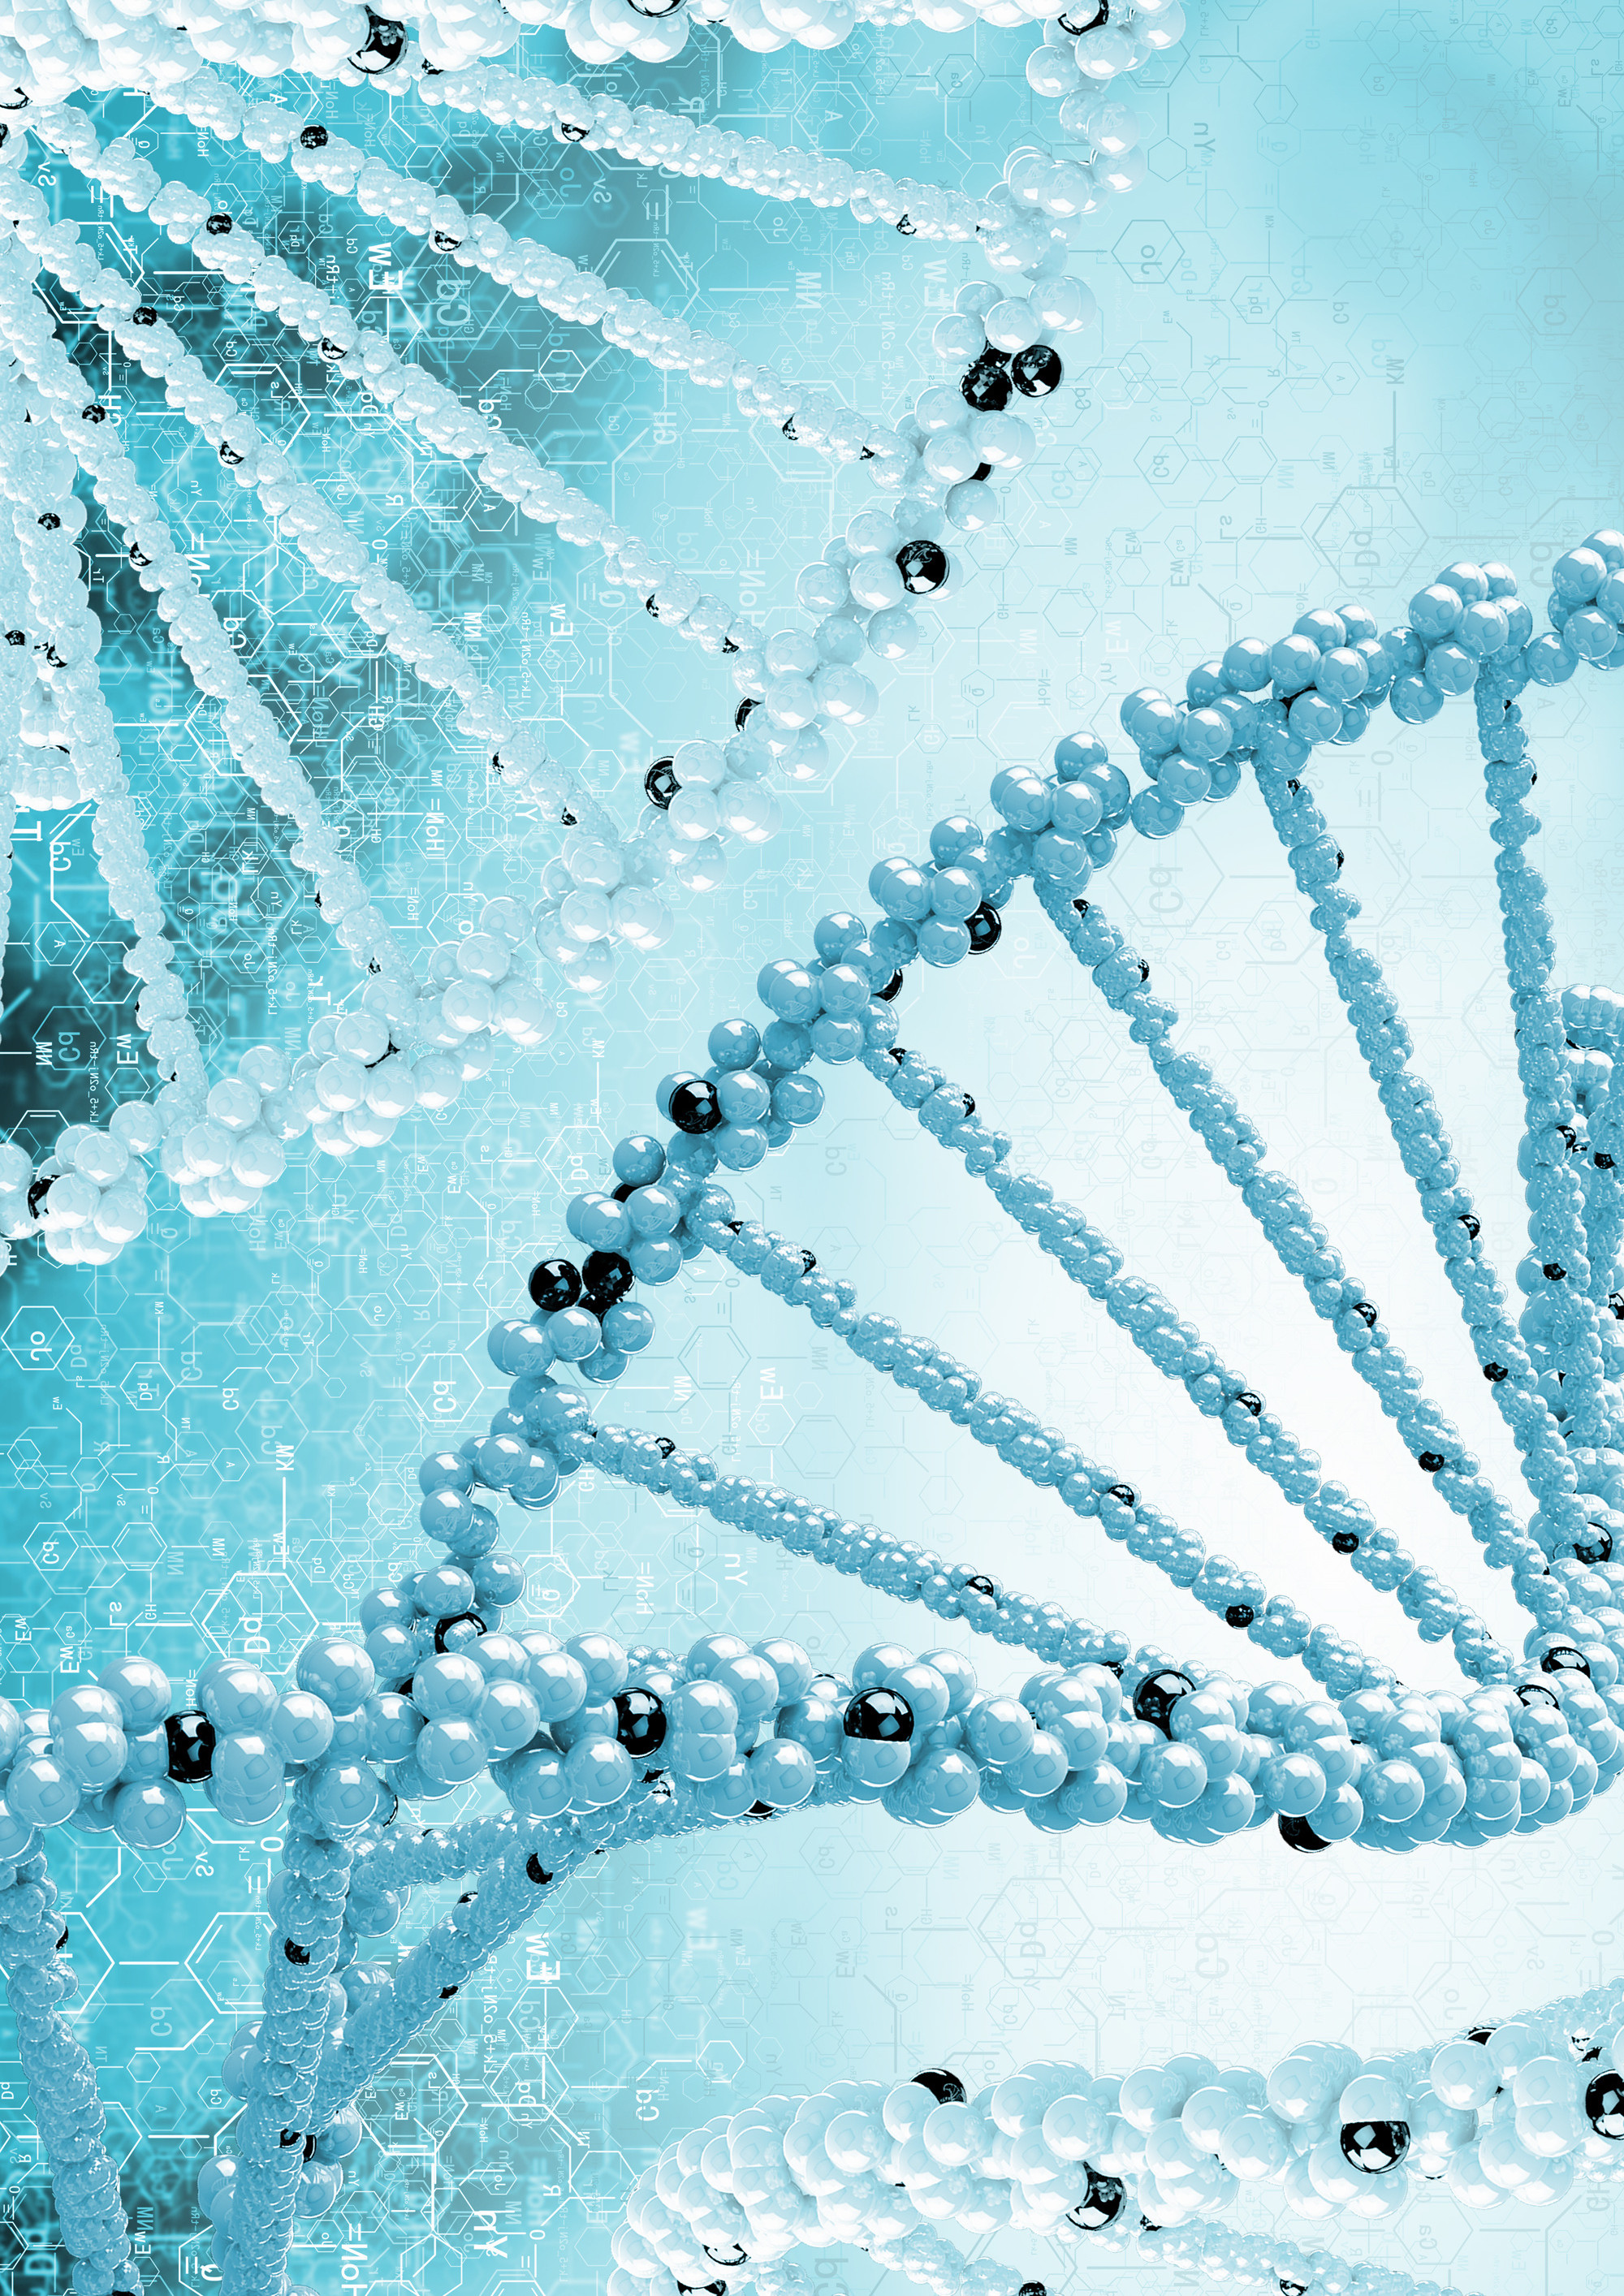
\includegraphics[width=\paperwidth,height=\paperheight]{../UTILS/Background/BG03_A0.png}}}

\usepackage[english, francais]{babel}
\selectlanguage{francais}

\addto\captionsfrancais{%
   \def\figurename{Figure}%
}
\addto\captionsfrancais{%
   \def\tablename{Table}%
}


\title{\huge{Développement et Application de Méthodologies Statistiques pour Etudes Longitudinales d'Association Génétique}\linebreak \large{\textit{Comité de suivi de thèse: première année}}}
\date{28 septembre 2015}
\email{\href{mailto:mickael.canouil@cnrs.fr}{mickael.canouil@cnrs.fr}}
\author{Mickaël Canouil}
\grade{Doctorant en Biostatistique}
\institute{\cmdb{G}énomique \cmdb{I}ntégrative et \cmdb{M}odélisation des \cmdb{M}aladies \cmdb{M}étaboliques \linebreak UMR 8199 (CNRS / Université de Lille 2 / Institut Pasteur de Lille)}
\address{CNRS UMR8199 - Institut de Biologie de Lille\linebreak
1 Rue du Professeur Calmette\linebreak
BP 245\linebreak
F-59019 LILLE CEDEX
}
\cst{
\textbf{Directeur de thèse:}\\ Pr. Philippe Froguel\\ \vskip 0.25cm
\textbf{Co-directeur de thèse:}\\ Dr. Ghislain Rocheleau (Lille 2)\\ \vskip 0.25cm
\textbf{Membres du CST:}\\ Dr. Hélène Jacqmin-Gadda (INSERM U 897, Bordeaux)\\
Pr. Cristian Preda (Ecole Polytechnique, Lille)
}

% <<title, echo = FALSE, results = hide>>=
% @


\begin{document}
\maketitle
\tableofcontents

\clearpage
\section{Introduction et contexte}
\par{La prévalence mondiale du diabète de type 2 (T2D) est en constante augmentation et génère par
le fait même des efforts soutenus dans la découverte de nouveaux marqueurs génétiques impliqués dans
le risque de la maladie \citep{world_health_organization_diabetes_2015}. Ces dernières années,
les études d’association pangénomiques (GWAS) ont identifié plusieurs variants génétiques associés
à des traits métaboliques et au T2D, dont pas moins de 65 loci associés à la susceptibilité du T2D \citep{morris_large-scale_2012}.
Les GWAS ont notamment identifié 36 variants associés à la glycémie à jeun chez des individus normoglycémiques \citep{dupuis_new_2010, scott_large-scale_2012}.
Bien que le rôle fonctionnel de la plupart de ces loci reste à déterminer, ils ont tout de même permis de mettre
en lumière des liens intéressants entre le glucose sanguin et le T2D, et souligné quelques différences entre
l’homéostasie du glucose dans la population générale et les niveaux physiopathologiques observés chez les diabétiques.
La majorité de ces loci ont été trouvés par méta-analyse de GWAS, malgré la très grande hétérogénéité
des études et des cohortes incluses dans la méta-analyse.}

\par{La grande majorité des GWAS publiées ont utilisé un design transversal plutôt qu’un design longitudinal.
Cependant, une étude prospective longitudinale offre la possibilité de mesurer une même variable plusieurs
fois au cours de l’étude, permettant également une description de ses fluctuations temporelles.
Il est attendu que la puissance de détecter des variants génétiques associés à ces variables soit augmentée
grâce aux multiples mesures prises à plusieurs moments, puisqu’elles donnent globalement plus d’information
qu’une seule mesure prise à un moment donné. De plus, un design longitudinal permet d’étudier les variants
associés aux changements (trajectoires) de ces mesures à travers le temps, tout en augmentant la puissance
de détecter des différences entre les groupes (définis par leur génotype, dans un contexte génétique).
Tout porte à croire qu’une bonne modélisation de ces trajectoires optimiserait les tests d’association et
permettrait une meilleure exploitation des phénotypes disponibles.}


\section{Objectif de la thèse}
\par{Cette thèse propose de développer et implémenter des approches pangénomiques basées sur
des modèles de régression, tels les modèles linéaires mixtes (LMM), les équations estimantes généralisées (GEE) \citep{sitlani_generalized_2015},
et les modèles joints (JM) liant de façon statistique la variation temporelle d’une variable (p.ex., glucose sanguin)
avec la survenue d’une maladie (p.ex., T2D). Ces approches pourraient mener à l’identification de nouveaux loci.
De plus, ces méthodologies permettront de confronter la vision actuelle selon laquelle les gènes impliqués
dans les niveaux de glucose chez les individus normoglycémiques diffèrent de ceux observés dans les niveaux
pathophysiologiques des sujets atteints de T2D \citep{yaghootkar_recent_2013}.
Aussi, ces approches statistiques appliquées à un contexte génétique pourraient permettre d’expliquer pourquoi
certains individus en légère hyperglycémie ne développent pas le T2D.
Les marqueurs ainsi identifiés renforceront du même coup l’utilité clinique de la stratification
génétique du risque dans la population générale \citep{pal_genetics_2013}.}

\par{Néanmoins, les approches LMM, GEE et JM nécessitent de grandes quantités de ressources lorsqu'appliquées
sur des millions de loci et des milliers d’individus.
Aussi, ces approches sont le plus souvent utilisées sur un sous-ensemble de loci dans des régions d’intérêts de la
pathologie étudiée \citep{beyene_longitudinal_2014, wu_longitudinal_2014}.
Des approches dites "rapides" ont été développées pour pallier au problème du temps de calcul, présents notamment sur les
implémentations actuelles des LMM (\cmd{nlme} et \cmd{lme4} pour R), et se basent sur des méthodes
d’approximation des LMM \citep{sikorska_fast_2013, sikorska_gwas_2015, sikorska_computationally_2014}.
A ce jour, deux implémentations des JM existent sur la plateforme CRAN pour le logiciel R \citep{Rsoftware}.
La première est développée par Dimitris Rizopoulos (\cmd{JM}) \citep{rizopoulos_jm_2010} et se focalise sur l’estimation des paramètres du
sous modèle de survie, quand la seconde, développée par Pete Philipson (\cmd{joineR}) \citep{philipson_joiner_2012}, vise à estimer principalement
les paramètres du sous modèle LMM.}


\section{Matériels}
\par{La cohorte prospective D.E.S.I.R (Données Épidémiologiques sur le Syndrome d’Insulino-Résistance),
comprend 5 214 sujets suivis pendant neuf années au cours desquelles plusieurs mesures
phénotypiques ont été prises à quatre occasions uniformément réparties durant la période de suivi (0, 3, 6 et 9 ans).
En exploitant l’approche par GWAS dans la cohorte D.E.S.I.R, une percée majeure a été réalisée dans la génétique
des traits métaboliques menant, d’une part, à la découverte de nouveaux loci associés au T2D, et d’autre part,
à l’identification de loci impliqués dans le glucose sanguin de sujets normoglycémiques \citep{dupuis_new_2010, voight_twelve_2010}.
La base de données phénotypique et génotypique existante de D.E.S.I.R offre l’opportunité unique de modéliser
la trajectoire temporelle de plusieurs phénotypes dont le glucose sanguin, et peut-être même permettra
de découvrir de nouveaux loci simultanément associés à l’incidence du T2D et à un taux élevé de glucose sanguin.}
\par{L’étude des données a été réalisée avec le logiciel R sur un serveur de calcul de 80 coeurs
et 500 Go de mémoire vive, accessible dans le laboratoire de l'unité UMR8199 dirigée par le Pr. Phlippe Froguel.}


\section{Méthodes\label{sec:Methods}}
\begin{figure}[ht]
    \begin{center}
        \fbox{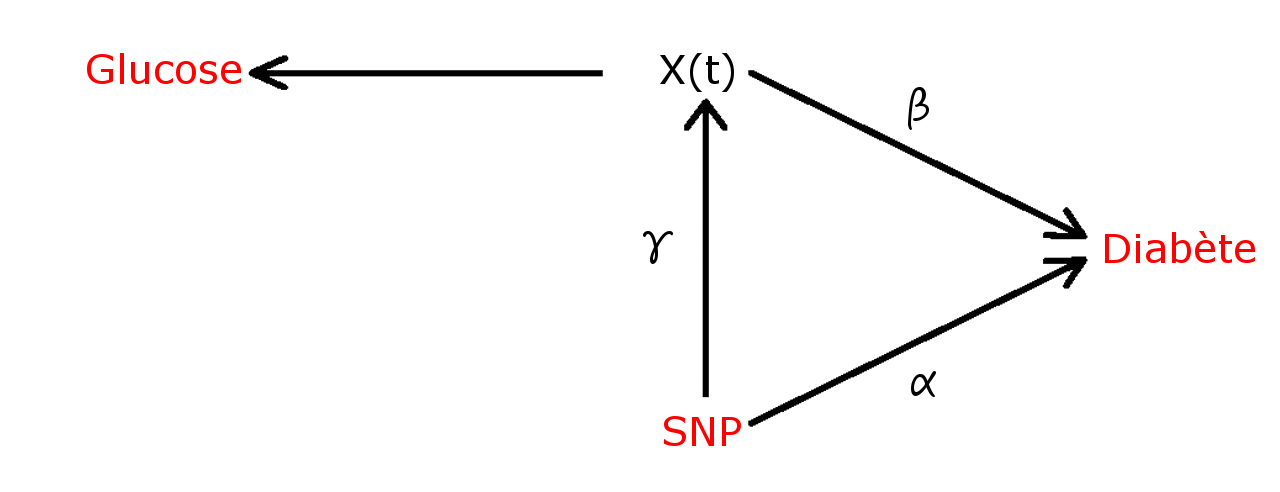
\includegraphics[width=15cm]{figures/jointModel.png}}
    \end{center}
    \vspace{-15pt}
    \caption{Diagramme général d'un modèle joint pour le T2D (adapté de \cite{ibrahim_basic_2010})\newline
    {\small $X(t)$: trajectoire de glucose sanguin inférée des données longitudinales observées;
    $\alpha$: effet du SNP sur le diabète;
    $\gamma$: effet du SNP sur la trajectoire de glucose sanguin;
    $\beta$: effet de la trajectoire de glucose sanguin sur le diabète.}}
    \label{fig:JointModel}
\end{figure}

\par{Le risque d’incidence de T2D a d’abord été évalué à l’aide d’un modèle de survie de Cox,
avec une variable dépendante du temps \citep{fisher_time-dependent_1999}, le glucose sanguin,
ainsi qu’une variable fixe non dépendante du temps, le SNP.
Pour un individu $i$ au temps $t$, la fonction de risque $\lambda_i(t)$ est exprimée par
\begin{eqnarray}\lambda_i(t)=\lambda_0(t)\times exp(\beta \times X_i(t)+\alpha \times SNP_i)\label{eq:1}\end{eqnarray}
où $\lambda_0(t)$ est la fonction de risque de base.
Le paramètre $\alpha$ représente l’effet du SNP sur le temps de survenue de l’événement,
quand $\beta$ est l’association entre la trajectoire de glucose sanguin et le temps du T2D.}
\par{Dans un second temps, les approches de type modèle joint ont été appliquées (paquet R: \cmd{JM} et \cmd{joineR}).
Les modèles joints intégrent deux composantes, une composante de survie (\bref{eq:1}{Equation}) et
une composante longitudinale, généralement modélisée par un modèle linéaire mixte
\begin{eqnarray}Y_{ij}=X_{ij}+\epsilon_{ij}\label{eq:2}\end{eqnarray}
avec $Y_{ij}$ la valeur observée, $X_{ij}$ la vraie valeur (non observée) de la variable longitudinale, et
$\epsilon_{ij}$ l’erreur de mesure pour l’individu $i$ au temps $j$, supposée normalement distribuée.
La variable $X_{ij}$ représente la trajectoire modélisée comme une fonction du temps (linéaire, quadratique, etc),
et peut inclure des covariables. Dans la suite du texte, nous supposons que
\begin{eqnarray}X_{ij}=\theta_{0i}+\theta_{1i}\times t_{ij}+\gamma \times SNP_i\label{eq:3}\end{eqnarray}
Nous supposons que les paramètres $\theta_{0i}$ et $\theta_{1i}$ suivent une loi normale bivariée.
Le paramètre $\gamma$ représente l’effet du SNP sur la trajectoire de glucose sanguin.}


\section{Résultats préliminaires}
\subsection{Cohorte D.E.S.I.R}
\par{Dans le but de tester les approches LMM et JM, des SNPs, découverts par méta-analyses de GWAS, associés
au glucose sanguin et au T2D (consortium \citeauthor{diagram_consortium} et \citeauthor{magic_consortium}), ont été sélectionnés.
Les individus présents dans la cohorte D.E.S.I.R ont pour la plupart (environ 4 500) été génotypés
à l’aide d’une Metabochip DNA arrays (Illumina) \citep{voight_metabochip_2012}.
Les approches précédemment décrites à la \bref{sec:Methods}{Section} ont été appliquées.
Il s’agissait ici de confirmer ces marqueurs génétiques dans la cohorte D.E.S.I.R, en incluant, dans un même modèle,
l'information d'incidence de T2D et le glucose sanguin.}
\setlength{\tabcolsep}{5pt}
\begin{table}[ht]
    \begin{center}
        \begin{tabular}{rcccccc}
            \hline
            & \multicolumn{2}{c}{$\gamma$} & \multicolumn{2}{c}{$\alpha$} & \multicolumn{2}{c}{$\beta$} \\
            & Estimation & Valeur-p & Estimation & Valeur-p & Estimation & Valeur-p \\
            \hline
                rs7903146\_A (TCF7L2) & \textcolor{dodgerblue}{0.02465} & \textcolor{dodgerblue}{1.2e-02} & 0.2204 & 0.0629 & \textcolor{firebrick2}{3.477} & \textcolor{firebrick2}{1.5e-53} \\
                rs3802177\_G (SLC30A8) & \textcolor{dodgerblue}{0.038} & \textcolor{dodgerblue}{1.2e-04} & 0.01066 & 0.9329 & \textcolor{firebrick2}{3.542} & \textcolor{firebrick2}{3.0e-55} \\
                rs7756992\_G (CDKAL1) & 0.01842 & 6.6e-02 & 0.08661 & 0.4651 & \textcolor{firebrick2}{3.511} & \textcolor{firebrick2}{5.2e-55} \\
                rs10278336\_G (GCK) & \textcolor{dodgerblue}{0.0383} & \textcolor{dodgerblue}{3.5e-05} & 0.09214 & 0.4197 & \textcolor{firebrick2}{3.527} & \textcolor{firebrick2}{1.7e-54} \\
                rs1552224\_A (ARAP1) & \textcolor{dodgerblue}{0.03644} & \textcolor{dodgerblue}{4.5e-03} & 0.1077 & 0.5177 & \textcolor{firebrick2}{3.529} & \textcolor{firebrick2}{1.5e-55} \\
                rs560887\_C (G6PC2) & \textcolor{firebrick2}{0.09504} & \textcolor{firebrick2}{1.2e-22} & \textcolor{dodgerblue}{-0.3237} & \textcolor{dodgerblue}{0.0076} & \textcolor{firebrick2}{3.568} & \textcolor{firebrick2}{9.4e-56} \\
                rs780094\_C (GCKR) & \textcolor{firebrick2}{0.06271} & \textcolor{firebrick2}{4.4e-12} & -0.09694 & 0.3938 & \textcolor{firebrick2}{3.568} & \textcolor{firebrick2}{2.8e-55} \\
                rs10830963\_G (MTNR1B) & \textcolor{firebrick2}{0.0959} & \textcolor{firebrick2}{4.1e-22} & \textcolor{dodgerblue}{-0.3868} & \textcolor{dodgerblue}{0.0021} & \textcolor{firebrick2}{3.611} & \textcolor{firebrick2}{8.5e-56} \\
                rs2075423\_G (PROX1) & \textcolor{dodgerblue}{0.02666} & \textcolor{dodgerblue}{4.0e-03} & -0.03139 & 0.7784 & \textcolor{firebrick2}{3.538} & \textcolor{firebrick2}{1.7e-55} \\
                rs10811661\_T (CDKN2A) & 0.01671 & 1.4e-01 & 0.0003004 & 0.9983 & \textcolor{firebrick2}{3.636} & \textcolor{firebrick2}{2.4e-55} \\
                rs11717195\_T (ADCY5) & \textcolor{dodgerblue}{0.02581} & \textcolor{dodgerblue}{1.8e-02} & -0.1202 & 0.3788 & \textcolor{firebrick2}{3.554} & \textcolor{firebrick2}{1.5e-55} \\
                rs4402960\_A (IGF2BP2) & 0.01174 & 2.3e-01 & 0.06249 & 0.5958 & \textcolor{firebrick2}{3.558} & \textcolor{firebrick2}{1.2e-55} \\
                rs6878122\_G (ZBED3) & 0.01349 & 1.6e-01 & -0.000382 & 0.9974 & \textcolor{firebrick2}{3.444} & \textcolor{firebrick2}{1.0e-54} \\
            \hline
        \end{tabular}
    \end{center}
    \vspace{-15pt}
    \caption{Résultat d'analyse pour une sélection de SNPs connus pour être associés au T2D ou au glucose sanguin.
    Résultats obtenus avec le paquet \cmd{JM} et ajustés à l'âge, au sexe et à l'IMC.
    {\small En \textcolor{dodgerblue}{bleu}, $\textrm{valeur-p}<0.05$ et en \textcolor{firebrick2}{rouge}, $\textrm{valeur-p}<5\times 10^{-8}$.}}
    \label{tab:desisrJM}
\end{table}\setlength{\tabcolsep}{10pt}
\par{Comme prévu, ces résultats confirment les résultats obtenus par GWAS (\bref{fig:gwas}{Figure}), notamment
la forte association entre le glucose sanguin et le SNP ($\gamma \neq 0$).
Les valeurs-p mises en évidence dans la \bref{tab:desisrJM}{Table} ne sont pas aussi petites que celles rapportées
dans la littérature, en raison de l'effectif réduit de la cohorte D.E.S.I.R, en comparaison des milliers d'individus
présents dans les méta-analyses de GWAS.
L'association entre la trajectoire du glucose et le risque d'incidence de T2D est très significative ($p<10^{-50}$), de par
la définition même de l'incidence de T2D (définie selon un seuil de glucose dans le sang supérieur à 7mM/L).
Rappelons que le seuil de significativité pangénomique est communément fixé à $5\times 10^{-8}$.}
\begin{figure}[ht]
    \begin{center}
        \fbox{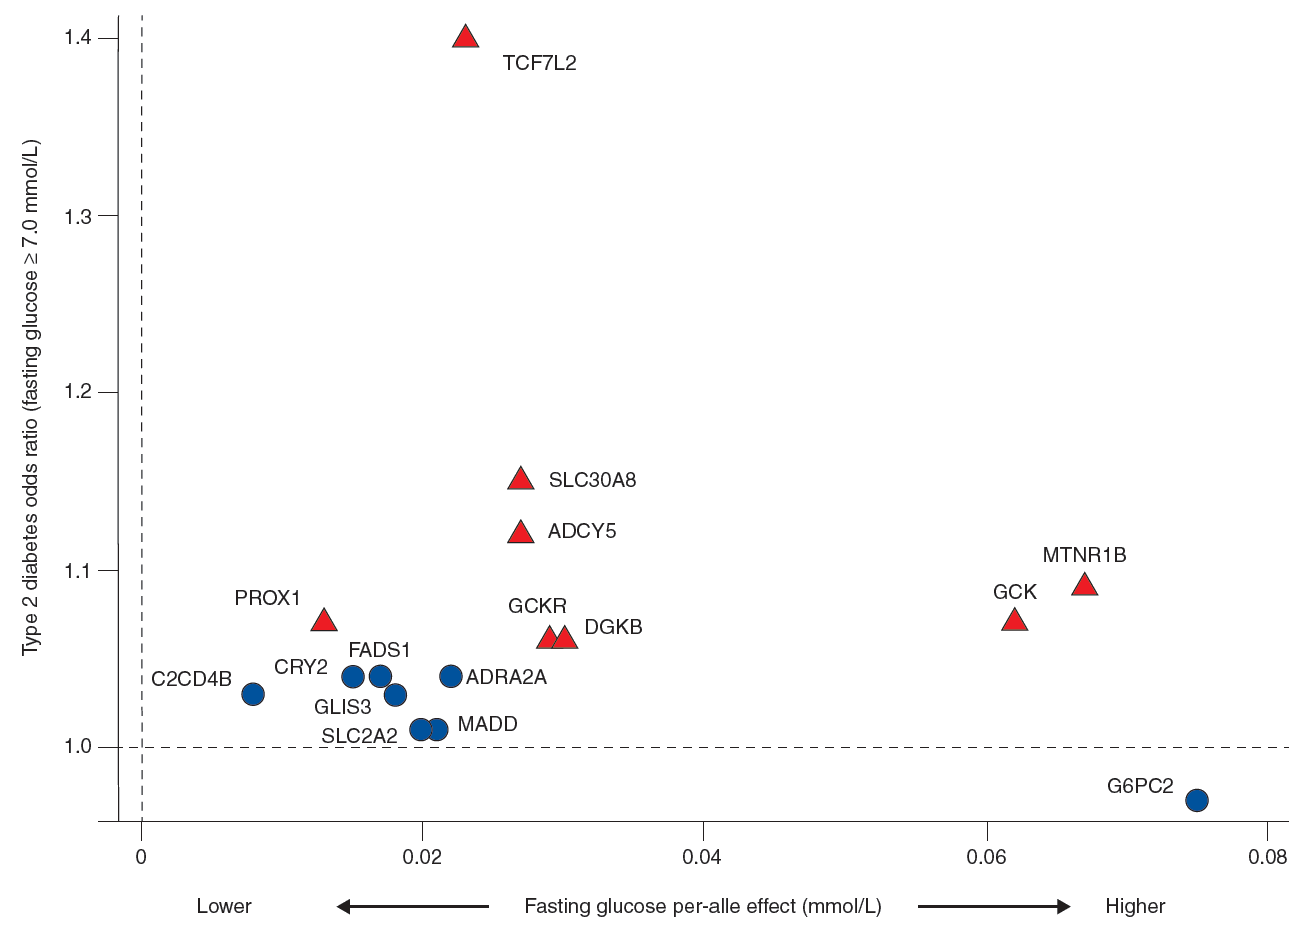
\includegraphics[width=15cm]{figures/Yaghootkar.png}}
    \end{center}
    \vspace{-15pt}
    \caption{Résultat d'association des allèles à risques pour le T2D et le glucose sanguin \citep{yaghootkar_recent_2013}.
    {\small \textcolor{dodgerblue}{Cercle bleu}: l'association au glucose sanguin pour $\textrm{valeur-p}<5\times 10^{-8}$;
    \textcolor{firebrick2}{Triangle rouge}: l'association au T2D et au glucose sanguin $\textrm{valeur-p}<5\times 10^{-8}$.}}
    \label{fig:gwas}
\end{figure}
% \par{L'approche par modèle joints permet d'identifier des marqueurs présentant à la fois un effet sur la
% trajectoire du glucose sanguin et sur le risque d'incidence de T2D.
% Dans cette optique, les résultats du gène G6PC2 sont prometteurs avec à la fois un effet sur la trajectoire du glucose
% (augmentation du glucose pour les porteurs de l'allèle à risque) et un effet sur l'incidence de T2D (réduction du risque).
% Ces résultats sont en accord avec les résultats de la \bref{fig:gwas}{Figure}, montrant le gène G6PC2 avec un Odd Ratio inférieur
% à un \citep{yaghootkar_recent_2013}.}
\par{Les données de la cohorte D.E.S.I.R ont également été analysées avec des approches classiques de LMM
(paquet \cmd{nlme}) et par une approche dite "Two-Step" (TS) \citep{self_modeling_1992}.
Cette dernière approche consiste en la succession de deux étapes:
\begin{description}
    \item[Etape 1] Ajustement d'un modèle linéaire mixte pour estimer la "vraie" trajectoire.
    \item[Etape 2] Ajustement d'un modèle de survie incorporant la trajectoire estimée de l'étape 1
    en tant que covariable dépendante du temps.
\end{description}
\setlength{\tabcolsep}{5pt}
\begin{table}[ht]
    \begin{center}
        \begin{tabular}{rcccccc}
            \hline
            & \multicolumn{2}{c}{$\alpha$} & \multicolumn{2}{c}{$\beta$} \\
            & Estimation & Valeur-p & Estimation & Valeur-p \\
            \hline
            rs7903146\_A (TCF7L2) & \textcolor{dodgerblue}{0.317} & \textcolor{dodgerblue}{1.0e-04} & \textcolor{firebrick2}{3.356} & \textcolor{firebrick2}{$<2\times 10^{-16}$} \\
            rs3802177\_G (SLC30A8) & 0.1291 & 1.5e-01 & \textcolor{firebrick2}{3.375} & \textcolor{firebrick2}{$<2\times 10^{-16}$} \\
            rs7756992\_G (CDKAL1) & \textcolor{dodgerblue}{0.1829} & \textcolor{dodgerblue}{2.4e-02} & \textcolor{firebrick2}{3.372} & \textcolor{firebrick2}{$<2\times 10^{-16}$} \\
            rs10278336\_G (GCK) & -0.1373 & 8.2e-02 & \textcolor{firebrick2}{3.376} & \textcolor{firebrick2}{$<2\times 10^{-16}$} \\
            rs1552224\_A (ARAP1) & 0.06174 & 5.8e-01 & \textcolor{firebrick2}{3.392} & \textcolor{firebrick2}{$<2\times 10^{-16}$} \\
            rs560887\_C (G6PC2) & \textcolor{dodgerblue}{-0.2725} & \textcolor{dodgerblue}{9.6e-04} & \textcolor{firebrick2}{3.432} & \textcolor{firebrick2}{$<2\times 10^{-16}$} \\
            rs780094\_C (GCKR) & -0.04382 & 5.8e-01 & \textcolor{firebrick2}{3.404} & \textcolor{firebrick2}{$<2\times 10^{-16}$} \\
            rs10830963\_G (MTNR1B) & \textcolor{dodgerblue}{-0.2683} & \textcolor{dodgerblue}{1.4e-03} & \textcolor{firebrick2}{3.456} & \textcolor{firebrick2}{$<2\times 10^{-16}$} \\
            rs2075423\_G (PROX1) & -0.1184 & 1.2e-01 & \textcolor{firebrick2}{3.407} & \textcolor{firebrick2}{$<2\times 10^{-16}$} \\
            rs10811661\_T (CDKN2A) & 0.03332 & 7.3e-01 & \textcolor{firebrick2}{3.364} & \textcolor{firebrick2}{$<2\times 10^{-16}$} \\
            rs11717195\_T (ADCY5) & -0.08409 & 3.7e-01 & \textcolor{firebrick2}{3.405} & \textcolor{firebrick2}{$<2\times 10^{-16}$} \\
            rs4402960\_A (IGF2BP2) & 0.09775 & 2.2e-01 & \textcolor{firebrick2}{3.391} & \textcolor{firebrick2}{$<2\times 10^{-16}$} \\
            rs6878122\_G (ZBED3) & 0.07204 & 3.7e-01 & \textcolor{firebrick2}{3.386} & \textcolor{firebrick2}{$<2\times 10^{-16}$} \\
            \hline
        \end{tabular}
    \end{center}
    \vspace{-15pt}
    \caption{Résultat d'analyse pour une sélection de SNPs connus pour être associés au T2D et au glucose sanguin.
    Résultats obtenus avec l'approche "Two-Step", ajustés à l'âge, au sexe et à l'IMC (paquets \cmd{nlme} et \cmd{survival}).\newline
    {\small En \textcolor{dodgerblue}{bleu}, $\textrm{valeur-p}<0.05$ et en \textcolor{firebrick2}{rouge}, $\textrm{valeur-p}<5\times 10^{-8}$}.}
    \label{tab:desisrTS}
\end{table}\setlength{\tabcolsep}{10pt}
L'approche TS présente des résultats proches de ceux obtenus par l'approche JM.
Néanmoins, l'estimation du paramètre $\beta$ est systématiquement inférieure à celle obtenue par \cmd{JM}.
L'estimation du paramètre $\alpha$ (effet du SNP sur l'incidence de T2D) diffère substantiellement de celle obtenue par le modèle joint.}
\par{L'approche TS permet de réduire le biais introduit par l'ajout d'une covariable dépendante du temps dans un
modèle de survie. Cependant, cette approche n'est pas sans biais, puisque l'information d'incidence de T2D
n'est pas intégrée dans l'estimation de la "vraie" trajectoire \citep{mccrink_advances_2013}.}

\clearpage
\subsection{Simulations}
\begin{table}[h]
    \begin{center}
        \begin{tabular}{lc}
            \hline
            Paramètres & Valeurs\\
            \hline
            Effectif ($N$) & $5000$\\
            Temps de mesures (en années) & $0, 3, 6, 9$\\
            Incidence à neuf ans ($I$) & $5\%$\\
            LMM : Trajectoire $\left (\begin{bmatrix}\theta_{0}\\\theta_{1}\end{bmatrix}\right )$ & $\mathcal{N}_2\left (\begin{bmatrix}4.50\\0.013\end{bmatrix} , \begin{bmatrix} 0.16 & 0 \\ 0 & 1\times 10^{-3} \end{bmatrix} \right )$\\
            LMM : Effet du SNP ($\gamma$) & $0.025$\\
            Cox : Effet du SNP ($\alpha$) & $0.2$\\
            JM : Effet de la trajectoire ($\beta$) & $3.50$\\
            \hline
        \end{tabular}
    \end{center}
    \vspace{-15pt}
    \caption{Paramètres initiaux pour la simulation des données. {\small Caractéristiques basées sur le SNP de TCF7L2 (SNP le plus fortement associé au T2D).}}
    \label{tab:simpar}
\end{table}
\par{Dans le but d’identifier les avantages et limites des approches de type modèle joint (\cmd{JM} et \cmd{joineR}),
un jeu de données a été simulé sur la base de la cohorte D.E.S.I.R.
Les jeux de données de simulation, qui ont été réalisés avec R, suivent les \hyperref[eq:1]{Equations~\ref*{eq:1}~à~\ref{eq:3}}
et les paramètres donnés dans la \bref{tab:simpar}{Table}.
La fonction de risque de base $\lambda_0$ a été fixée de façon à obtenir une incidence équivalente à celle de
la cohorte D.E.S.I.R (environ 5\%), durant la période de suivi de neuf ans.}
\par{Plusieurs scénarios de simulation ont été réalisés pour tester la robustesse des estimations des paramètres
en présence de données manquantes, en utilisant la classification usuelle:}
\begin{description}
    \addtolength{\itemindent}{1cm}
    \item[MCAR (missing completely at random):] les données sont manquantes indépendamment des données observées et non observées;
    \item[MAR (missing at random):] conditionnellement aux données observées, les données manquantes sont indépendantes des données non observées;
    \item[MNAR (missing not at random):] les données manquantes sont dépendantes de variables non observées.
\end{description}
\par{D’autres paramètres ont également été étudiés, tels que l’effectif de la population,
la fréquence du marqueur génétique et dans le cas plus général des LMM, le nombre de mesures longitudinales.
Ces scénarios ont été étudiés avec les paquets \cmd{JM} et \cmd{joineR}.}
\par{Les scénarios adoptés et étudiés avec les paquets \cmd{JM} et \cmd{joineR} sont les suivants:
\begin{enumerate}
    \addtolength{\itemindent}{1cm}
    \item Données complètes et variation de la fréquence allélique;
    \item Données complètes et variation du nombre de mesures longitudinales;
    \item Données complètes et variation de l'effectif;
    \item Données manquantes distribuées de façon uniforme (MCAR);
    \item Perte au suivi (MCAR);
    \item Données manquantes conditionnellement au génotype (MAR);
    \item Données manquantes conditionnellement à une variable non observée (MNAR). (Scénario non encore implémenté).
\end{enumerate}
}
\par{En raison de la complexité du calcul, un faible nombre de simulations (1000) a été réalisé pour produire
les figures suivantes.}

\subsubsection{Scénario 1: variation de la fréquence allélique\label{sec:S1}}
\begin{figure}[ht]
    \begin{center}
        \fbox{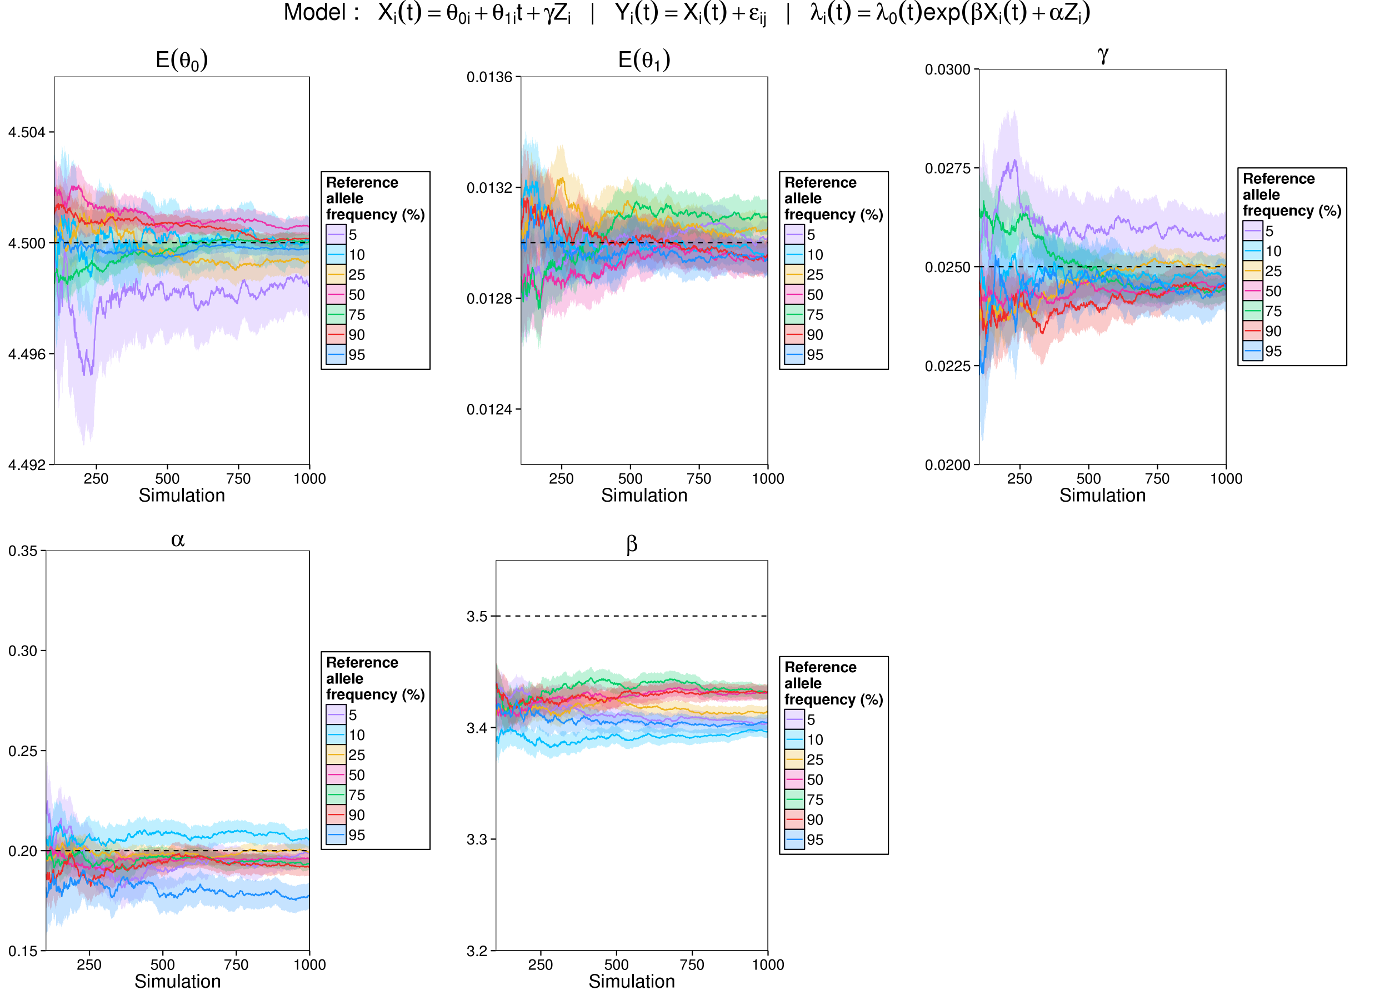
\includegraphics[width=15cm]{figures/S1_JM.png}}
    \end{center}
    \vspace{-15pt}
    \caption{Estimation par \cmd{JM} (Scénario~1).}
    \label{fig:S1JM}
\end{figure}
\par{Ces premières simulations (\bref{fig:S1JM}{Figure}) révèlent que \cmd{JM} ne semble pas présenter de biais
important pour l’estimation des paramètres liés au LMM.
Il en va de même pour le paramètre $\alpha$ du modèle de survie, ce qui était attendu: en effet,
\cmd{JM} se focalise sur l’estimation des paramètres de la composante de survie du modèle joint.
Néanmoins, l’estimation du $\beta$, issue du modèle de survie de JM, est sous-estimée de façon systématique dans ce scénario.
La fréquence allélique semble influencer, de façon plus ou moins importante, l'estimation des paramètres lorsque celle-ci est faible ($f<5\%$).}
\begin{figure}[ht]
    \begin{center}
        \fbox{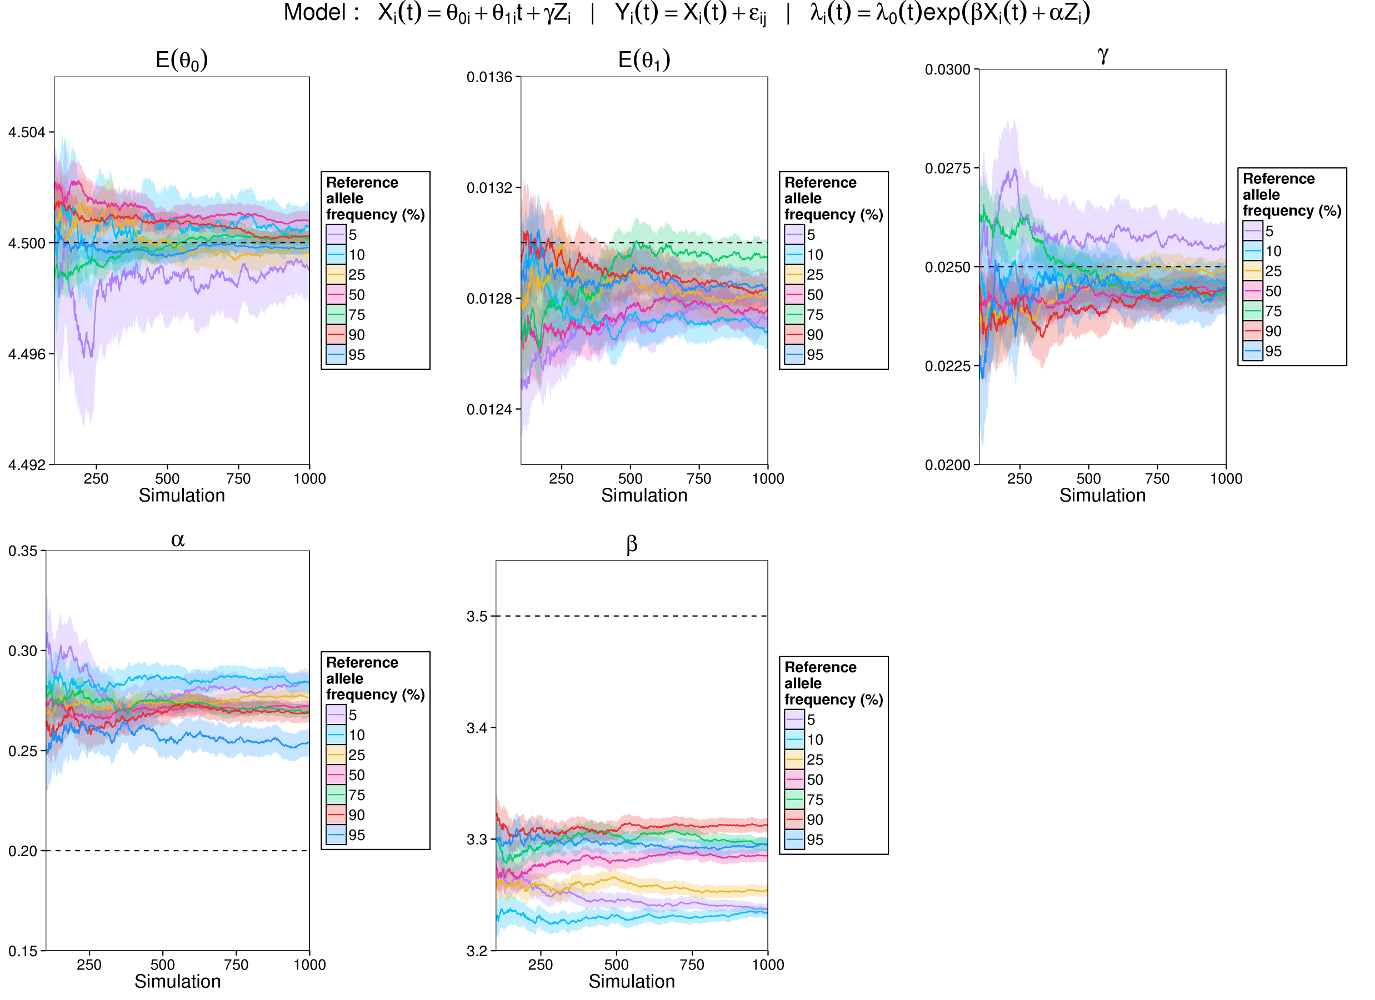
\includegraphics[width=15cm]{figures/S1_joineR.png}}
    \end{center}
    \vspace{-15pt}
    \caption{Estimation par \cmd{joineR} (Scénario~1).}
    \label{fig:S1joineR}
\end{figure}
\par{Dans le cas des estimations obtenues à l’aide de \cmd{joineR} (\bref{fig:S1joineR}{Figure}),
qui se focalise principalement sur les paramètres de la composante LMM, les estimations semblent non biaisées
pour $E(\theta_0)$ et $\gamma$. Cependant, sur les 1000 simulations réalisées, un biais sur le paramètre $E(\theta_1)$
est présent, en comparaison du biais de l'estimation de \cmd{JM}.}
\par{En ce qui concerne la composante de survie, les estimations de $\alpha$ (l’effet du SNP) et de $\beta$
(l’effet de la trajectoire) sont respectivement surestimées et sous-estimées. Encore une fois, la fréquence allélique
ne doit pas être trop faible pour l'estimation des paramètres du modèle, notamment pour les paramètres de la composante
de survie.}

\subsubsection{Scénario 2: variation du nombre de mesures longitudinales\label{sec:S2}}
\begin{figure}[ht]
    \begin{center}
        \fbox{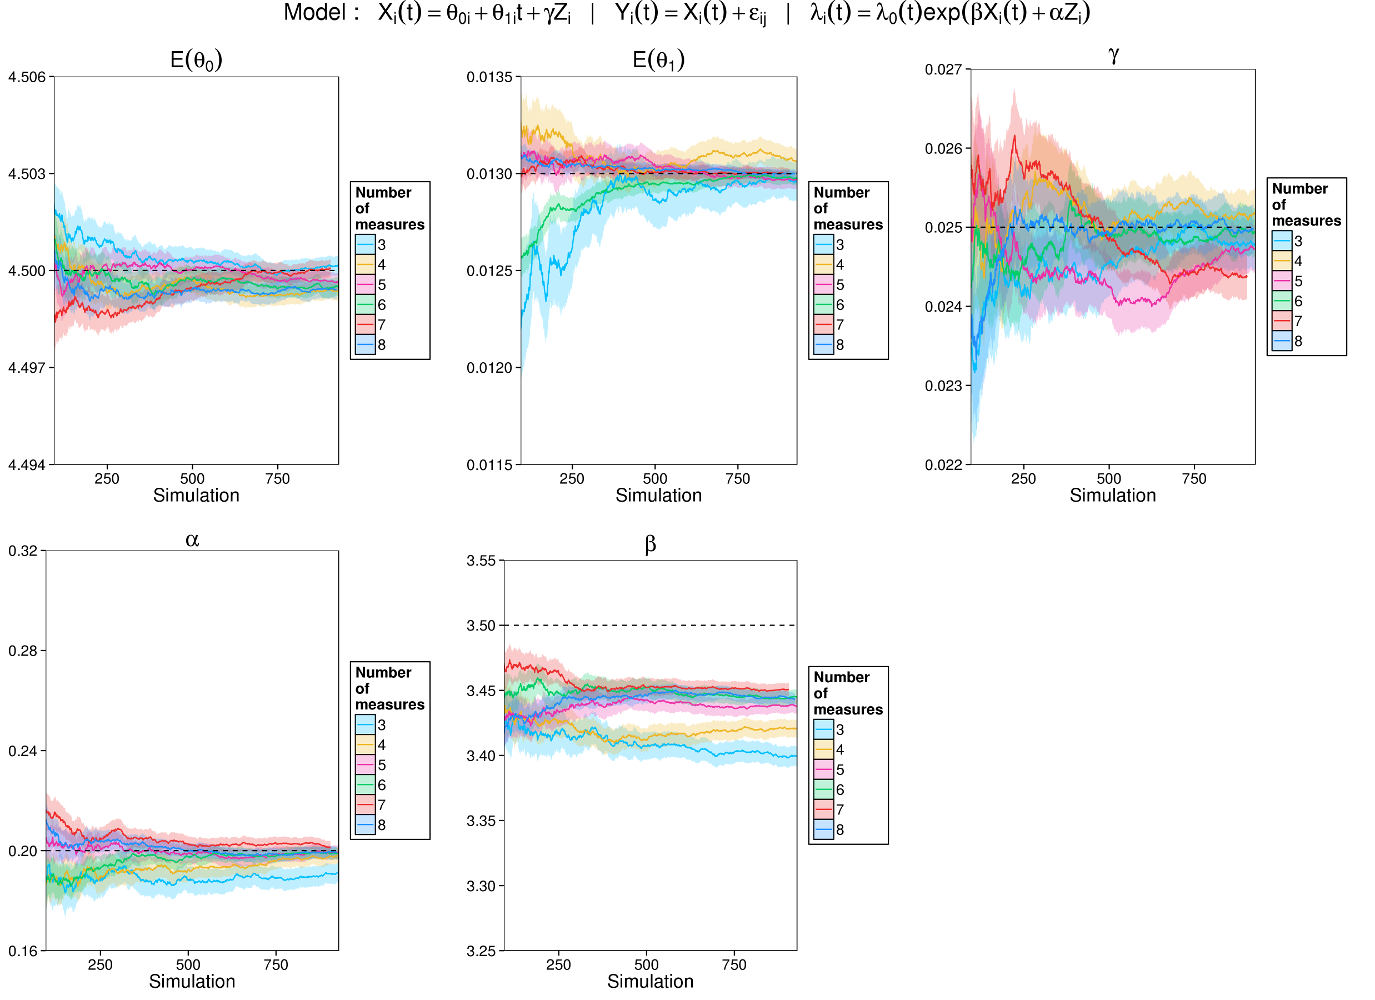
\includegraphics[width=15cm]{figures/S2_JM.png}}
    \end{center}
    \vspace{-15pt}
    \caption{Estimation par \cmd{JM} (Scénario~2).}
    \label{fig:S2JM}
\end{figure}
\par{En ce qui concerne \cmd{JM}, la variation du nombre de mesures ne révèle que peu de changement concernant
les paramètres de la composante LMM (\bref{fig:S2JM}{Figure}).
Le changement le plus notable réside dans l’estimation du paramètre $\beta$ de l’effet de la trajectoire
sur la survenue de l’évènement.
En effet, malgré le faible nombre de simulations, le biais de l’estimation se réduit avec l'augmentation du nombre
de mesures.}
\begin{figure}[ht]
    \begin{center}
        \fbox{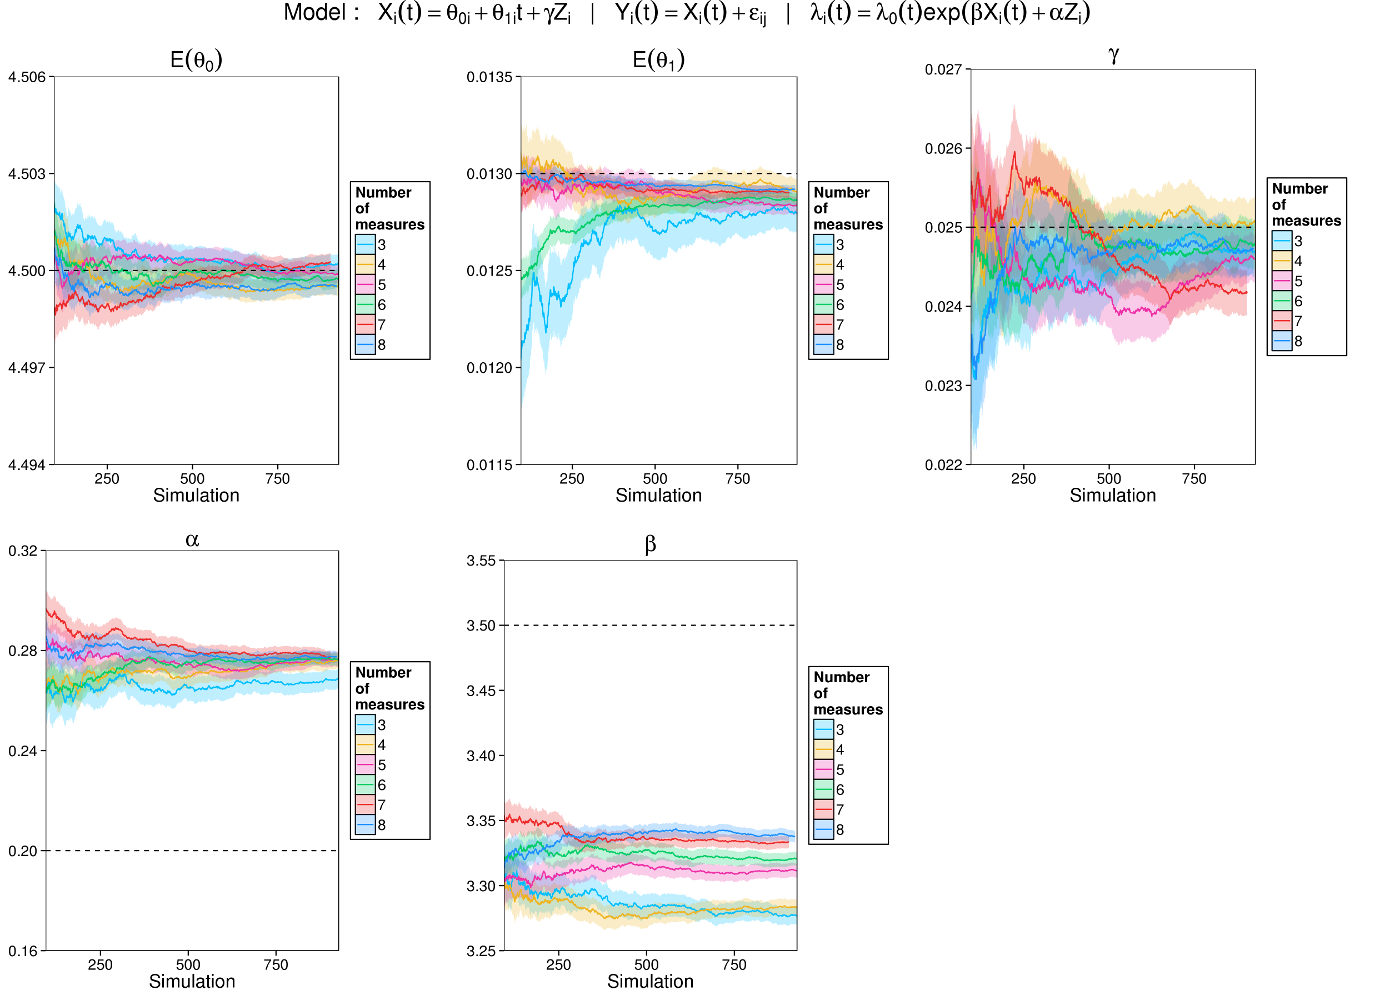
\includegraphics[width=15cm]{figures/S2_joineR.png}}
    \end{center}
    \vspace{-15pt}
    \caption{Estimation par \cmd{joineR} (Scénario~2).}
    \label{fig:S2joineR}
\end{figure}
\par{Le biais des estimations de \cmd{joineR} (\bref{fig:S2joineR}{Figure}) reste plus important que celui de \cmd{JM},
même si celui-ci se réduit avec l'augmentation du nombre de mesures longitudinales.
Cependant, le biais d'estimation de $\alpha$ varie très peu selon le nombre de mesures.
L'estimation de $E(\theta_1)$ demeure légèrement biaisée dans ce scénario, malgré le fait que le paquet \cmd{joineR} se concentre principalement
sur l'estimation des paramètres issus de la composante longitudinale du modèle joint.
Ce phénomène peut être dû à des problèmes de convergence, pouvant être causés par l'algorithme utilisé (par défaut)
dans \cmd{joineR}, à savoir \cmd{nlminb} du paquet \cmd{stats}.}

\subsubsection{Conclusion}
\par{Ces simulations ont permis de mettre en évidence des points forts et des points faibles des implémentations actuelles
des modèles joints (\cmd{JM} et \cmd{joineR}), et de se familiariser avec le processus de simulation des données.
Le biais des estimateurs devra être étudié de façon plus approfondie dans la suite de la thèse.}
\par{Une étude détaillée des algorithmes sera nécessaire pour mieux comprendre ces deux implémentations et
plus fondamentalement les modèles joints.
En effet, le raffinement de l'algorithme de simulation pourra permettre de mieux caractériser le biais observé (\hyperref[sec:S1]{Section~\ref*{sec:S1}~et~\ref{sec:S2}}).
Les scénarios de simulation de données manquantes (MCAR, MAR et MNAR) ont pour la plupart déjà été implémentés
et seront étudiés prochainement.}
\par{Les implémentations actuelles sont peu appropriées en terme de temps de calcul et ce, malgré l'utilisation d'un serveur de
calcul. En effet, 1000 simulations pour les scénarios présentés en \hyperref[sec:S1]{Section~\ref*{sec:S1} et~\ref{sec:S2}}
ont demandé environ 15 heures en pleine charge (80 Coeurs).
Au cours de la thèse, un effort plus important sera fourni dans l'amélioration du temps de calcul.}


\clearpage
\section{Perspectives}
\subsection{En cours / À court terme}
\par{
\begin{enumerate}
    \item Ecriture d’un article de revue de littérature sur les méthodes d’analyses de données longitudinales dans le contexte des études pangénomiques.
    \item Développement et raffinement des méthodes de simulation dans un contexte génétique:
    \begin{enumerate}
        \item fonction de risque par intervalles pour la composante de survie;
        \item extension aux modèles de Weibull, Gompertz, etc;
        \item caractérisisation du biais de l’estimation des paramètres dans \cmd{JM} et \cmd{joineR}.
    \end{enumerate}
\end{enumerate}
\subsection{À long terme}
Développement et implémentation de solutions:
\begin{itemize}
    \item pour réduire le temps de calcul;
    \item pour réduire le biais des estimations.
\end{itemize}
}


\clearpage
\section{Formations}
\subsection{Passées}
\par{
\begin{itemize}
    \item Formation Collège doctoral: \textit{Gérer efficacement sa documentation avec ZOTERO} (20 février 2015).
    \item Participation (poster) et obtention d’une bourse SFD-Lilly au \textit{Congrès annuel de la SFD} (Société Francophone du Diabète) du 24 au 27 mars 2015,
    à Bordeaux.
    \item Formation Collège doctoral: \textit{Veille et stratégie de recherche documentaire} (08 avril 2015).
    \item Participation et animation d’un atelier Julia lors des \textit{JDEV 2015
    (Journées nationales du DEVeloppement logiciel de l'Enseignement Supérieur et Recherche)},
    du 20 juin au 3 juillet, à Bordeaux.
    \item Ecole doctorale: participation au \textit{comité d'organisation de la Journée André Verbert} 2015 (14 septembre 2015).
\end{itemize}
Nombre de crédits obtenus à ce jour: 9/60 crédits.
}

\subsection{Futures}
\par{
\begin{itemize}
    \item Formation Collège doctoral: \textit{LaTex Niveau avancé}.
    \item Formation Collège doctoral: \textit{Déposer, signaler et diffuser sa thèse : ce qu'il faut savoir}.
    \item Formation Collège doctoral: \textit{Améliorer ses chances d'être publié : Pourquoi ? Comment ?}
    \item \textit{Congrès de la SFD 2016} (Société Francophone du Diabète)
    \item \textit{Congrès IGES 2016} (International Genetic Epidemiology Society)
    \item \textit{Rencontres R 2016}
    \item \textit{useR 2016}.
    \item Formation Collège doctoral: \textit{Accroître son aisance à l'oral grâce aux approches théâtrales}.
    \item ...
\end{itemize}
}



% \setlength{\tabcolsep}{10pt} % default
\clearpage
\addcontentsline{toc}{section}{Références}
\bibliographystyle{apalike}
\bibliography{CST2015.bib}
% \nocite{*}


% \appendix
% \setcounter{table}{0}
% \setcounter{figure}{0}
% \renewcommand\thetable{\alph{table}}
% \renewcommand\thefigure{\alph{figure}}
% \clearpage

\end{document}